\documentclass[a4paper,10pt,epsf,fleqn]{article}
\usepackage{makeidx}
\makeindex
\setlength{\mathindent}{0mm}
\usepackage{graphicx}
\oddsidemargin=1cm\pagebreak[2]
\topmargin=-1cm
\setlength{\textwidth}{15cm}
\setlength{\textheight}{24cm}
\pagestyle{plain}

\newcommand{\rou}[1]{\noindent------------------------------------------------------------------------------------------------------------

\noindent{\bf \large #1}}
\newcommand{\fl}[1]{\noindent{\sf $\bullet$ #1\index{\sf #1}} : }
\newcommand{\fx}[1]{\subsection{\sf #1\index{\sf #1}}}
\newcommand{\ssx}[1]{\subsection{\bf #1\index{\bf #1}}}
\newcommand{\ssxx}[2]{\subsection{\bf #1\index{\bf #2}}}
\newcommand{\infiles}{\noindent\fbox{Input files}}
\newcommand{\outfiles}{\noindent\fbox{Output files}}

\begin{document}
\baselineskip=6mm
\title{All-electron GW code applicable to FP-LMTO and other methods.}
\author{Takao Kotani and Mark van Schilfggarde}
%\date{April 2nd 2001}
\maketitle
\tableofcontents

\vspace{5mm}
\noindent$\bullet${\bf Reference}

\vspace{5mm}
\noindent$\bullet${\bf Index of I/O fies, shel scripts and executions.}

\newpage
\section{Introduction}
We will explain a new all-electron $GW$ code.
As for the inputs for the $GW$ calculation, 
we have to supply the eigenfunctions and the eigenvalues
in addition to the crystal-structure informations.
The eigenfuncion should be expanded by
the two-kind of basis functions,
the atomic functions in the muffin-tin(MT) spheres and
the planewaves in the interstitial region.
The GW code is applicable not only to FP-LAPW but also for FP-LMTO,
because the envelope functions used in the method are also well expanded
by the plane wave in the interstitial region. 
The Coulomb matrix $v$, the dynamically screened
Coulomb interaction $W$, and so on, are expanded in a mixed basis set
which consists of the two contributions, 
the local atom-centered functions confined to MT spheres, 
and the interstitial plane wave (IPW), which is defined as
the plane waves with the overlap to the local
functions projected out.
The local functions are calculated from products of
solutions to the Schr\"odinger equation within the
MT sphere, and can include any of the core states.
Thus, the core functions can be treated on an equal footing
with the valence electrons.
In addiion, we include the all the energy dependence of $W$.
The code is developed from the GW code by Ferdi Aryasetiawan for LMTO-ASA.
We added some improvements in addition to the mixed-basis feature.

You can get the package {\tt ecal.001.tar.gz} which contains FP-LMTO developed by Mark,
and the GW codes. Please contact {\tt kotani@phys.sci.osaka-u.ac.jp}.
Now we also have samples {\tt ecal.001.tar.gz}, though we will gather datas 
in a web site in future.


%%%%%%%%%%%%%%%%%%%%%%%%%%%%%%%%%%%%%%%%%%%%%%%%%%%%%%%%%%%%%%%%%%%%%%%%%%%%%%%%
\newpage
\section{Overview of $GW$ calculation}
The Hedin's $GW$ gives the self-energy as
\begin{equation} 
\label{self_energy}
\Sigma({\bf r},{\bf r}^{\prime},\omega)=\frac{i}{2\pi}\int d\omega'
G({\bf r},{\bf r}^{\prime},\omega+\omega^{\prime})e^{i\delta\omega^{\prime}}
W({\bf r},{\bf r}^{\prime},\omega^{\prime}),
\end{equation}
where $W$ is the screened Coulomb interaction, and $G$ is the Green's
function. Our $GW$ calculation uses the onebody non-interacting Green function as $G$,
and the RPA screeened Coulomb interaction as $W$.
We can calculate these $G$ and $W$ directly from
the eigenvalues and eigenfunctions given by LDA.
Then the quasi-particle (QP) energy $E_n({\bf k})$ 
($n$ is the band index and ${\bf k}$ is the wave vector) is given by
\begin{equation}\label{quasiparticle_energy}
E_n({\bf k})=\epsilon_n({\bf k})+Z_{n{\bf k}}[\langle\Psi_{{\bf k}n}|
\Sigma({\bf r},{\bf r}^{\prime},\epsilon_n({\bf k}))|\Psi_{{\bf k}n}\rangle
- \langle\Psi_{{\bf k}n}|V_{\rm xc}^{\rm LDA}({\bf r})|\Psi_{{\bf k}n}\rangle],
\end{equation}
where $\epsilon_n({\bf k})$ and $\Psi_{{\bf k}n}$ denote the LDA
eigenvalues and eigenfunctions,
%and $\Sigma({\bf r},{\bf r}^{\prime},\epsilon_n({\bf k}))$ denotes the
%$GW$ self-energy.
and the QP renormalization factor
$Z_{n{\bf k}}$ is
\begin{equation}\label{Renormalization}
Z_{n{\bf k}}=[1-\langle\Psi_{{\bf k}n}|
\frac{\partial}{\partial\omega} \Sigma({\bf r},{\bf r}^{\prime},
\epsilon_n({\bf k}))|\Psi_{{\bf k}n}\rangle]^{-1}.
\end{equation}
The $GW$ gives the QP energies based on Eq.(\ref{quasiparticle_energy}).
(However, our calculations seem to show that better agreements are obtained
when we set $Z=1$ in Eq.(\ref{quasiparticle_energy}). See argument in Sec.\ref{zeq1ornot}.)

Both in FP-LAPW and FP-LMTO, space is devided into
the muffin-tins (MT) and the interstial region.
The eigenfunctions $\Psi^{{\bf k}n}({\bf r})$ can be
expanded by the linear combination of local atomic orbitals
$A_{au}({\bf r}) \equiv \{ \phi_{aL}(r) Y_L(\hat{\bf r}),\dot{\phi}_{aL}(r) Y_L(\hat{\bf r}) \}$
within MTs.
Here $\phi_{aL}(r)$ and $\dot{\phi}_{aL}(r)$ denote 
the normalized-orthogonal basis 
constructed from the solutions of the radial Schr\"odinger equations
($\dot{\phi}$ does not need to be the energy derivative).
$u \equiv(L, I_{\rm P})$ is the composite index
where $I_{\rm P}$ takes 1 for $\phi$, or 2 for $\dot{\phi}$.
$a$ is the index to specify atom in the primitive cell and
${\bf R_a}$ denotes its position measured from the center of the cell.
$A_{au}({\bf r})$ makes normalized-orthogonal in each MT $a$.
Then the eigenfunction $\Psi^{{\bf k}n}$ is expanded as
\begin{eqnarray}
\label{eigenfunction}
\label{psieq}
\Psi^{{\bf k}n}({\bf r}) 
= \sum_{a u} \alpha^{{\bf k} n}_{au} A^{\bf k}_{a u}({\bf r})
 + \sum_{\bf G} \beta^{{\bf k}n}_{\bf G} P^{\bf k}_{\bf G}({\bf r}),
\end{eqnarray}
where we use the interstitial plane wave (IPW) defined as
\begin{eqnarray}
P^{\bf k}_{\bf G}({\bf r}) &=& 0  \ \ \ {\rm \ if \ {\bf r} \in any \ MT} \nonumber \\
        &=&   \exp (i ({\bf k+G}) {\bf r}) \ \ \ {\rm otherwise},
\end{eqnarray}
and the Bloch sums of $A_{a u}$
\begin{eqnarray}
A^{\bf k}_{a u}({\bf r}) &\equiv& \sum_{\bf T} A_{a u}({\bf r-R_a-T}) \exp(i {\bf kT}).
\end{eqnarray}
${\bf T}$ means the posions of all the cell centers (translation vectors).

Through Eq.(\ref{psieq}), the products $\Psi_{{\bf k_1}n} \times \Psi_{{\bf k_2}n'}$ can
be expanded by $P^{\bf k_1+k_2}_{\bf G}({\bf r})$
in the interstitial region because
$P^{\bf k_1}_{\bf G_1}({\bf r}) \times P^{\bf k_2}_{\bf G_2}({\bf r})=
P^{\bf k_1+k_2}_{\bf G_1+G_2}({\bf r})$.
The products also expanded within the MT sphere $a$
by $B_{am}^{\bf k_1+k_2}({\bf r})$, which is the Bloch sum of
the product basis $B_{am}({\bf r})$, which in turn are constructed
from the products of $A_{au}({\bf r}) \times A_{au'}({\bf r})$
following the procedure by Aryasetiawan\cite{aryasetiawan94}.

We define the mixed basis
$\{M^{\bf k}_I({\bf r}) \}\equiv \{ P^{\bf k}_{\bf G}({\bf r}), B_{am}^{\bf k}({\bf r})\}$,
where the index $I\equiv \{ {\bf G},am\}$ classifies the members of the basis.
As a result, $M^{\bf k}_I$ is a good basis set in the expansion of the products.
The complete information to calculate the self-energy and $E_n({\bf k})$ are
the matrix elements of the products $\langle \Psi_{{\bf q}n}| \Psi_{{\bf q-k}n'} M^{\bf k}_I \rangle$,
the LDA eigenvalues $\epsilon_{{\bf k}n}$, 
the Coulomb matrix $v_{IJ}({\bf k})
\equiv \langle M^{\bf k}_{I} |v|  M^{\bf k}_{J} \rangle$, 
and the overlap matrix $\langle M^{\bf k}_I |  M^{\bf k}_{I} \rangle$.
(The overlap matrix of IPW is necessary because
 $\langle P^{\bf k}_{\bf G} |  P^{\bf k}_{\bf G'} \rangle \ne 0$
for ${\bf G} \ne {\bf G}'$.)
The Coulom interaction is expanded as
\begin{eqnarray}
\label{coulombexpand}
v({\bf r},{\bf r}') &=& 
\sum_{{\bf k},I,J} |\tilde{M}^{\bf k}_I \rangle
v_{IJ}({\bf k}) \langle \tilde{M}^{\bf k}_J|,
\end{eqnarray}
where we define
\begin{eqnarray}
|\tilde{M}^{\bf k}_{I} \rangle &\equiv& \sum_{I'}
|M^{\bf k}_{I'} \rangle \langle M^{\bf k}_{I'} |  M^{\bf k}_I \rangle^{-1}.
\end{eqnarray}
$W$ and the polalization function $D$ below are expanded
in the same manner of Eq.(\ref{coulombexpand}).
The exchange part of the self-energy is written as
\begin{eqnarray}
\langle \Psi_{{\bf q}n}|\Sigma_{\rm x} |\Psi_{{\bf q}n} \rangle
&&=\sum^{\rm BZ}_{{\bf k}}  \sum^{\rm  occ}_{n'}
\langle \Psi_{{\bf q}n}| \Psi_{{\bf q-k}n'} \tilde{M}^{\bf k}_I \rangle 
v_{IJ}({\bf k})
\langle \tilde{M}^{\bf k}_J \Psi_{{\bf q-k}n'} | \Psi_{{\bf q}n} \rangle. \label{sx}
\end{eqnarray}
The screened Coulomb interaction $W_{IJ}({\bf q},\omega)$ is calculated
through $W = (1-v D)^{-1} v$, where the polarization function $D$ is
\begin{eqnarray}
D_{IJ}({\bf q},\omega)
&&=\sum^{\rm BZ}_{{\bf k}}  \sum^{\rm  occ}_{n} \sum^{\rm  unocc}_{n'}
\langle \tilde{M}^{\bf q}_I \Psi_{{\bf k}n} |\Psi_{{\bf q+k}n'} \rangle
\langle \Psi_{{\bf q+k}n'}| \Psi_{{\bf k}n} \tilde{M}^{\bf q}_J \rangle \nonumber \\
&& \times
(\frac{1}{\omega-\epsilon_{{\bf q+k}n'}+\epsilon_{{\bf k}n}+i \delta}
-\frac{1}{\omega+\epsilon_{{\bf q+k}n'}-\epsilon_{{\bf k}n}-i \delta}). \label{dieele}
\end{eqnarray}
We use the tetrahedron method for the Brillouin zone (BZ) summation in Eq.(\ref{dieele})
following Ref.~\cite{rath75}.
Then the correlation part of $\Sigma$ is
\begin{eqnarray}
\langle \Psi_{{\bf q}n}|\Sigma_{\rm c}(\omega) |\Psi_{{\bf q}n} \rangle
&& = \sum^{\rm BZ}_{\bf k}  \sum^{\rm  All}_{n'} \sum_{IJ}
\langle \Psi_{{\bf q}n}| \Psi_{{\bf q-k}n'} \tilde{M}^{\bf k}_I \rangle
\langle \tilde{M}^{\bf k}_J \Psi_{{\bf q-k}n'} | \Psi_{{\bf q}n} \rangle  \nonumber \\
&& \times \int_{-\infty}^{\infty} \frac{i d\omega'}{2 \pi}
W^{\rm c}_{IJ}({\bf k},\omega')
\frac{1}{\omega'+\omega-\epsilon_{{\bf q-k}n'} \pm i \delta}. \label{sc}
\end{eqnarray}
Here $-i \delta$ is for occupied states; $+i \delta$ is for unoccupied
states.  $W^{\rm c} \equiv W - v$. We use the $\omega'$-integral method 
deviced by Aryasetiawan\cite{aryasetiawanasa1}: the integration path is deformed from
the real-axis to the imaginary axis so as not to across poles.
As a result,the integral is evaluated with the one along the imaginary axis plus
some additional contributions from the poles; see Fig.\ref{omegapath}.  
As for the method of the BZ summation used in Eqs.(\ref{sx},\ref{sc}), 
See section \ref{bzsums}.

In usual $GW$ calculations, 
Eq.(\ref{quasiparticle_energy}) is evaluated through
\begin{equation}\label{qpgwnc}
E_n({\bf k})=\epsilon_n({\bf k})+Z_{n{\bf k}}[\langle\Psi_{{\bf k}n}|
\Sigma^{\rm valence}({\bf r},{\bf r}^{\prime},\epsilon_n({\bf k}))|\Psi_{{\bf k}n}\rangle
- \langle\Psi_{{\bf k}n}|V_{\rm xc}^{\rm LDA}([n_{\rm valence}],{\bf r})|\Psi_{{\bf k}n}\rangle].
\end{equation}
Here $\Sigma^{\rm valence},V_{\rm xc}^{\rm LDA}([n_{\rm valence}])$ means that it does not contain
core contributions---Core-contributions are completely neglected.
In addition to this valence-only calculation, our code can
calculate $E_n({\bf k})$ including the core contributions through
\begin{eqnarray}
E_n({\bf k})=\epsilon_n({\bf k})+
Z_{n{\bf k}}\times [\langle\Psi_{{\bf k}n}|
\Sigma_{\rm x}^{\rm core1}({\bf r},{\bf r}^{\prime})+
\Sigma_{\rm xc}^{\rm core2+valence}({\bf r},{\bf r}^{\prime},\epsilon_n({\bf k}))|\Psi_{{\bf k}n}\rangle \nonumber \\
- \langle\Psi_{{\bf k}n}|V_{\rm xc}^{\rm LDA}([n_{\rm total}],{\bf r})|\Psi_{{\bf k}n}\rangle],
\label{qpgw}
\end{eqnarray}
where we devide all the cores into two groups, {\bf core1} and {\bf core2}.
{\bf core1} inculdes the deep cores and only affects
through the exchange self-energy. {\bf core2} includes relatively shallow
ones and treated on the same footing of the valence electrons.
This procedure, which is sugested by Aryasetiawan, works well; as for the deep cores,
it affects little on the results whether they are classified into {\bf core1} or {\bf core2}.
\begin{figure}
%\begin{center}
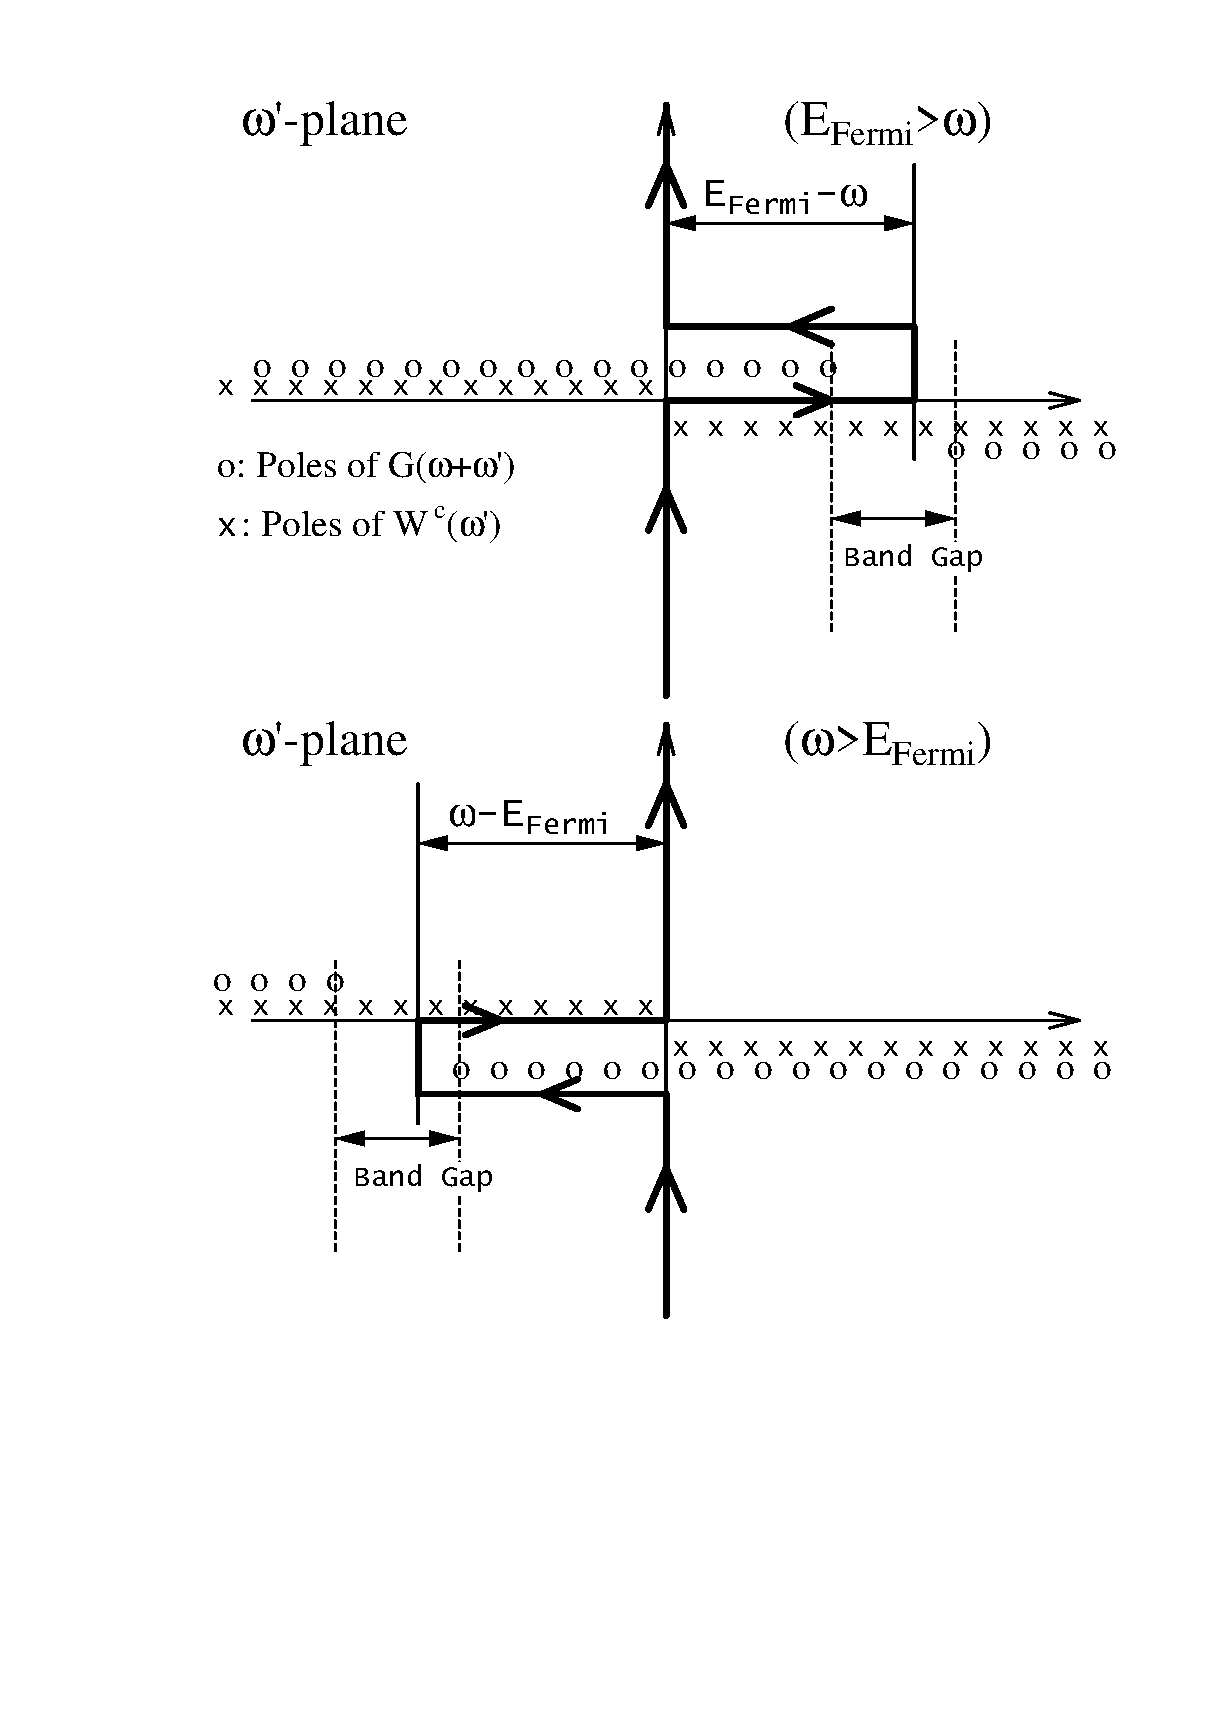
\includegraphics[width=11cm]{omegapath.eps} \label{omegapath}
%\end{center}
\caption[]{The integration contour of the correlated part of the self-energy,Eq.(\ref{sc}).
$G({\bf q-k},\omega'+\omega)= \sum_{n} {1}/{(\omega'+ \omega- \epsilon_{{\bf q-k}n})}$ 
has poles at $\omega'=\epsilon_{{\bf q-k}n}-\omega$. }
\label{omegapath}
\end{figure}



%%%%%%%%%%%%%%%%%%%%%%%%%%%%%%%%%%%%%%%%%%%%%%%%%%%%%%%%%%%%%%%%
\newpage
\section{Brillouin-zone integral for the self-energy; 
the smearing method + the offsetted $\Gamma$-point method.}
\label{kint}
     In Eqs.(\ref{sx},\ref{sc}), our smearing method means that 
each pole specified by $\epsilon_{{\bf q}-{\bf k} n'}$ is
treated as a uniform pole distribution
between $\epsilon_{{\bf q}-{\bf k} n'} \pm 0.5 E_{\rm smear}$.
In order to make things clear,
we explain in the case of $\Sigma_{\rm x}$ through Eqs.(\ref{sx}).
By the smering method,  Eqs.(\ref{sx}) is reduced to be
\setlength{\mathindent}{-8mm}
\begin{eqnarray}
&&\langle \Psi_{{\bf q}n}|\Sigma_{\rm x} |\Psi_{{\bf q}n} \rangle
= \sum_{\bf k}^{\rm 1st BZ} \rho_{{\bf q}n}({\bf k}), \label{sxqn}\\
&&\rho_{{\bf q}n}({\bf k}) \equiv \sum^{\rm  all}_{n'} \sum_{IJ}
\bar{\theta}(E_{\rm F}-\epsilon_{{\bf q- k} n'})
\langle \Psi_{{\bf q}n}| \Psi_{{\bf q-k}n'} \tilde{M}^{\bf k}_I \rangle v_{IJ}({\bf k})
\langle \tilde{M}^{\bf k}_J \Psi_{{\bf q-k}n'} | \Psi_{{\bf q}n} \rangle,
\label{sxsmear2}
\end{eqnarray}
where $\bar{\theta}$ is a smeared step function with $E_{\rm smear}$ written as
\setlength{\mathindent}{-5mm}
\begin{eqnarray}
&&\bar{\theta}(E_{\rm F}-\epsilon) = 1 \hspace{.5cm} {\rm for} \hspace{.3cm} \epsilon < E_{\rm F} - 0.5 E_{\rm smear} \nonumber \\
&&\hspace{1.3cm}= \frac{E_{\rm F} + 0.5 E_{\rm smear} -\epsilon}{E_{\rm smear}}  \hspace{.5cm}
{\rm \ for \ }  E_{\rm F} - 0.5 E_{\rm smear}<\epsilon<E_{\rm F} + 0.5 E_{\rm smear} \nonumber \\
&&\hspace{1.3cm}=0 \hspace{.5cm} {\rm \ for \ } E_{\rm F}+0.5 E_{\rm smear}<\epsilon.
\end{eqnarray}
\setlength{\mathindent}{0mm}
$E_{\rm smear}$ corresponds to the temperature cutoff, and $\bar{\theta}(E_{\rm F}-\epsilon)$
corresponds to the Fermi distribution function.
$\rho_{{\bf q}n}({\bf k})$ can have unsmooth behevior as a function of $k$ 
in BZ due to the Fermi energy cutoff. 
Larger $E_{\rm smear}$ reduce the unsmoothness.

$v_{IJ}({\bf k})$ is a periodic function in BZ,
and includes a singular part 
$v^0_{IJ}({\bf k})= A U^{0*}_I({\bf k}) U^{0}_J({\bf k}) F({\bf k})$
where $F({\bf k}) = 1/|{\bf k}|^2$ at ${\bf k} \to 0$.
$U^{0}_J({\bf k})$ deontes the corresponding normalized eigenfunction.
$F({\bf k})$ and $U^{0}_J({\bf k})$ are arbitrary except the singular behevior at ${\bf k} \to 0$.
Then we have
\begin{eqnarray}
&&\langle \Psi_{{\bf q}n}|\Sigma_{\rm x} |\Psi_{{\bf q}n} \rangle
= \sum_{\bf k}^{\rm 1st BZ} (\rho_{{\bf q}n}({\bf k}) - \rho^0_{{\bf q}n}({\bf k}))
 +\sum_{\bf k}^{\rm 1st BZ}  \rho^0_{{\bf q}n}({\bf k}), \label{sxdecomp}\\
&&\rho^0_{{\bf q}n}({\bf k})
 = A F({\bf k}) \sum^{\rm  all}_{n'} \sum_J \bar{\theta}(E_{\rm F}-\epsilon_{{\bf q- k} n'})
| U^{0}_J({\bf k}) \langle \tilde{M}^{\bf k}_J \Psi_{{\bf q-k}n'} | \Psi_{{\bf q}n} \rangle |^2.
\end{eqnarray}
As for the first term of right-hand side (RHS) of Eq.(\ref{sxdecomp}), 
the integrant $\rho_{{\bf q}n}({\bf k}) - \rho^0_{{\bf q}n}({\bf k})$
is a smooth function in BZ. Therefore, we can evaluate it
with a BZ discrete mesh, which is given as
\begin{eqnarray}
{\bf k}(i_1,i_2,i_3)= 2 \pi (\frac{i_1}{N_1} {\bf b}_1 
+ \frac{i_2}{N_2} {\bf b}_2 + \frac{i_3}{N_3} {\bf b}_3)
\label{kmesh}
\end{eqnarray}
where $i_1$ takes from 0 to $N_1-1$, $i_2$ from 0 to $N_2-1$, and $i_3$ from 0 to $N_3-1$.
Vectors $\{ {\bf b}_i| i=1,3\}$ givs the inverse of
the primitive translation vectors as ${\bf a}_i \cdot {\bf b}_j= \delta_{ij}$,
where $\{ {\bf a}_i| i=1,3\}$ denotes the translation vector.
The first term of RHS in Eq.(\ref{sxdecomp}) is evaluated with the replacement,
\begin{eqnarray}
\sum_{\bf k}^{\rm 1st BZ} \to \frac{1}{N_1N_2N_3} \sum_{i_1,i_2,i_3}.
\end{eqnarray}

As for the second term of RHS of Eq.(\ref{sxdecomp}),
we can choose $F({\bf k})$ so that $\rho^0_{{\bf q}n}({\bf k})= A' \tilde{F}({\bf k})$,
which is an analytic function
\begin{eqnarray}
\tilde{F}({\bf k})=\sum^{\rm All}_{\bf G} \frac{\exp(-\alpha |{\bf q + G}|^2) }{|{\bf q + G}|^2 },
\end{eqnarray}
where ${\bf G}$ denotes all the inverse reciprocal vertors and $\alpha$ is a parameter.
$A'$ is determined so as to keep the singular behevior of the socond term.
[Apparently, $\tilde{F}({\bf k})$ is positive definite, periodic in BZ and has the singular behevior at ${\bf k} \to 0$.
No problem to choose $F({\bf k})$.]
Then we can evaluate the second term analytically.
In the case of $\Sigma_{\rm x}$, it is not so difficult to calculate $A'$, however,
it get tremendous in the case of $\Sigma_{\rm c}$. The offsetted $\Gamma$-point method below
is to evalulate Eq.(\ref{sxdecomp}) without the evalualtion of $A'$.

The ofsetted $\Gamma$-point method means a BZ sum method with
\begin{eqnarray}
\sum_{\bf k}^{\rm 1st BZ} \to \frac{1}{N_1N_2N_3} \widetilde{\sum_{i_1,i_2,i_3}} \label{newmesh},
\end{eqnarray}
where $\widetilde{\sum}$ denotes the sum for ${\bf k}(i_1,i_2,i_3)$, but we
replace ${\bf k}(0,0,0)$ with the Q point of ${\bf Q}=(Q,0,0)$.
It is near $(0,0,0)$ and chosen so as to satisfy
\begin{eqnarray}
\sum_{\bf k}^{\rm 1st BZ} \tilde{F}({\bf k}) =
\frac{1}{N_1N_2N_3} \widetilde{\sum_{i_1,i_2,i_3}} \tilde{F}({\bf k}).
\end{eqnarray}
Apparently, we can calculate the second term of RHS of
Eq.(\ref{sxdecomp}) exactly with this mesh.
For larger $N_1N_2N_3$, $(Q,0,0)$ is closer to $(0,0,0)$,
then we can also use this mesh even for the first term of the RHS of Eq.(\ref{sxdecomp}) 
with little error.
Then Eq.(\ref{sxdecomp}) is reduced to be
\begin{eqnarray}
&&\langle \Psi_{{\bf q}n}|\Sigma_{\rm x} |\Psi_{{\bf q}n} \rangle
= \widetilde{\sum_{i_1,i_2,i_3}} (\rho_{{\bf q}n}({\bf k}) - \rho^0_{{\bf q}n}({\bf k})) 
 +\widetilde{\sum_{i_1,i_2,i_3}} \rho^0_{{\bf q}n}({\bf k})= \widetilde{\sum_{i_1,i_2,i_3}} \rho_{{\bf q}n}({\bf k}).
\end{eqnarray}
This means we just need to evaluate Eq.(\ref{sxqn}) with the mesh of Eq.(\ref{newmesh}).
In the practical application, we have to take some Q points so as to keep
the crystal symmetry. In addition, we use
\begin{eqnarray}
&&\rho_{{\bf q}n}({\bf Q}) \approx \sum^{\rm  all}_{n'} \sum_{IJ}
\bar{\theta}(E_{\rm F}-\epsilon_{{\bf q} n'})
\langle \Psi_{{\bf q}n}| \Psi_{{\bf q}n'} \tilde{M}^{\bf k=0}_I \rangle v_{IJ}({\bf Q})
\langle \tilde{M}^{\bf k=0}_J \Psi_{{\bf q}n'} | \Psi_{{\bf q}n} \rangle.
\end{eqnarray}


We have to take the two limit $E_{\rm smear} \to 0$ and
$N_1N_2N_3\to \infty$.
There could be a convergence problem as for
the states $\Psi_{{\bf q}n}$ whose $\epsilon_{{\bf q} n}$
are near $E_{\rm F}$ in the case of low DOS at $E_{\rm F}$.
In Fig.\ref{extestcab6}, we showed
the convergence test
for $\langle \Psi_{{\bf q}n}|\Sigma_{\rm x} |\Psi_{{\bf q}n} \rangle$
as a function of $E_{\rm smear}$ in the case of CaB$_6$.
The DOS at $E_{\rm Fermi}$ for CaB$_6$ is quite small, therefore,
it is a severe test for the smering method.
Through the comparison between 444 and 666 case, 
we can say a rapid change at $E_{\rm smear}\to 0$ will be
virtual because of the finite number of k points.
Therefore we can use $E_{\rm smear} \sim 0.05$ Ry
in order to avoid such a finite number effect at $E_{\rm smear}\to 0$.
Then we can expect 0.1 eV level of accuracy under the assumption of the flat
behevior at $E_{\rm smear}\to 0$.
Due to the calcellation effects, $\Sigma_{\rm x} + \Sigma_{\rm c}$ can
give better convergences.
\begin{figure}
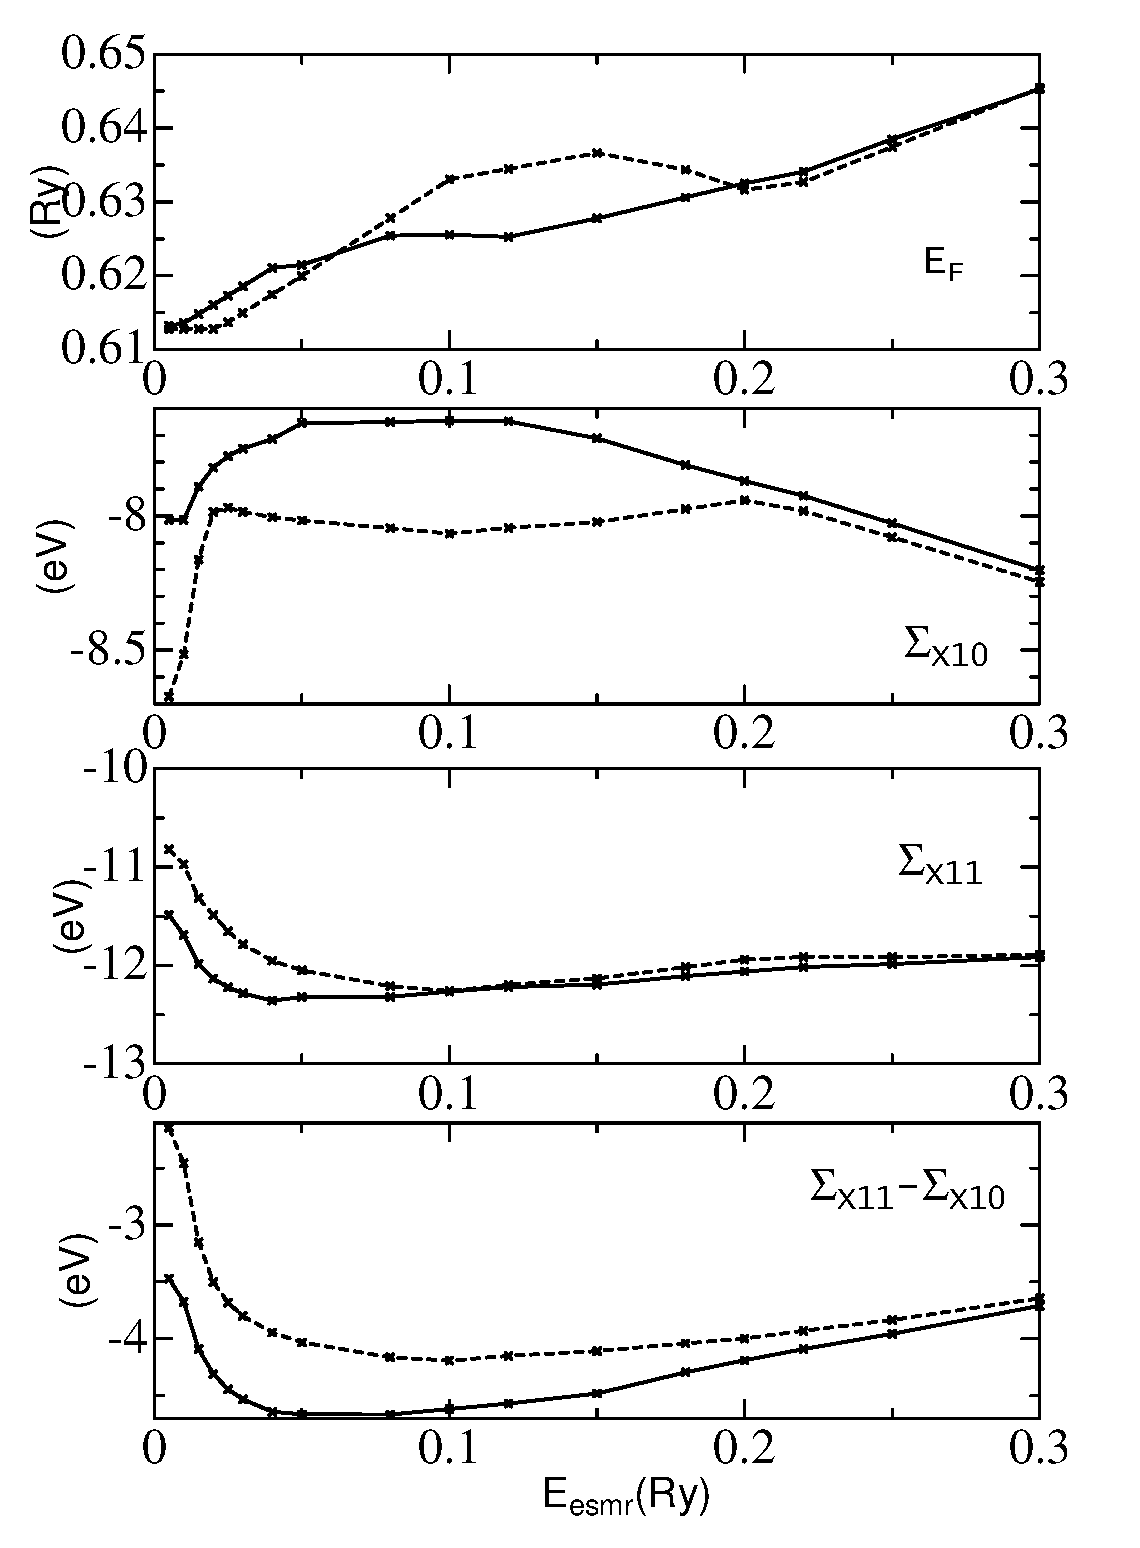
\includegraphics[width=15cm]{extest.eps}
\caption[]{$\langle \Psi_{{\bf q}n}|\Sigma_{\rm x} |\Psi_{{\bf q}n} \rangle$
as fucntions of $E_{\rm smear}$ for CaB$_6$, whose LDA bands are metallic.
the state $X_{10}$ is the top of the valence bands, and $X_{11}$ is the
bottom of the conduction bands. Solid line are for 666 case.
Broken lines are for 444 case. }
\label{extestcab6}
\end{figure}



%%%%%%%%%%%%%%%%%%%%%%%%%%%%%%%%%%%%%%%%%%%%%%%%%%%%%%%%%%%%%%%%%%%%%%%%
\newpage
\section{Whether the renomalization factor
Z is included or not in order to evaluate the quasi-particle energies?}
\label{zeq1ornot}

The quasi-particle energy(QPE) could be defined as the peak of
the spectrum function
$A(k,\omega)=  1/\pi \times |{\rm Im} ( G(k,\omega) ) |$ 
along the real $\omega$ axis.

In the commonly used method of $GW$, $G(k,\omega)$ is given as
$G(k,\omega) = 1/( \omega- e_k - \Sigma(k,\omega) )$,
where $e_k$ is given by LDA and $\Sigma(k,\omega)$ 
is also calculated from the LDA eigenfunctions and eigenvalues.
Then the peak position of $\omega $ is calculated so that its 
denominator=0, that is, $E_k - e_k - {\rm Re}\Sigma(k,E_k) =0$ (we set $\omega=E_k$).
Then the resulting expression of $E_k$ 
should include the renomalization factor $Z$.
We denote this method as the method (I). In (I), $\Sigma(k, E_k, [G])$
is approximated by $\Sigma(k, E_k, [G_{LDA}])$.
Here $[G]$ means that $\Sigma$ is a functional of $G$.

On the other hand, there might be an another method (II)
to get the QPE, where we simply evalulate the energy shift as
$\langle \psi_{k}| \Sigma(k, e_k) - V^{\rm xc}_{\rm LDA}| \psi_{k} \rangle$.
It corresponds to set $Z=1$.
Our calculations show that (II) gives better agreements
to experiments for the band gaps.
In (II), $\Sigma(k, E_k, [G])$ 
is approximated by $\Sigma(k, e_k, [G_{LDA}])$.

A widely used method (III), which is beyond these first-order methods (I) and (II),
is the method where we make the QPE self-consistent
with keeping the eigenfuncions as the ones give by LDA.
It is relatively easy and we might expect that
(III) gives some improvements than (I) and (II).
As a simplified version of (III), we can use the method (IV)
where we keep the screened Coulomb interaction $W$ as the one give by LDA.
It means that we assume that $W$ is well described by the LDA one.
Under the assumption that the method (IV) is good for QPE,
our question is reduced to be
'Which method (I) or (II) gives the better agreemets with (IV)?'

We show that not (I) but (II) well approximates (IV)
through a simple example.
We consider two states model whose LDA eigenvalues and eigenfunctions
are given by $\phi_1,e1$, and $\phi_2,e_2$.
The Fermi energy $E_{\rm f}$ is $e_2>E_{\rm f}>e_1 $. So $e_1$ is occupied and
$e_2$ is unoccupied. Then the Green function is written as
\begin{eqnarray}
G_{\rm LDA}(\omega) =   \frac{|\phi_1\rangle\langle\phi_1|}{\omega - e_1 -i\epsilon}
          + \frac{|\phi_2\rangle\langle\phi_2|}{\omega - e_2 +i\epsilon}.
\end{eqnarray}
$G$ given by (IV) is also given with some shifts of 
these eigenvalues, that is,
\begin{eqnarray}
G(\omega) =   \frac{|\phi_1\rangle\langle\phi_1|}{\omega - E_1 -i\epsilon}
            + \frac{|\phi_2\rangle\langle\phi_2|}{\omega - E_2 +i\epsilon}.
\end{eqnarray}
Then $E_1$ should be given by
\begin{eqnarray}
E_1 = e_1 + {\rm Re}\langle\phi_1|\Sigma(E_1,[G])- V^{\rm LDA}_{\rm xc}|\phi_1\rangle
\end{eqnarray}
and the same also for $E_2$.
If only the diagonal elements
$W_1(\omega)=\langle\phi_1 \phi_1|W(\omega) |\phi_1 \phi_1\rangle$
and $W_2(\omega)=\langle\phi_2 \phi_2|W(\omega) |\phi_2 \phi_2\rangle$
are important, the $GW$ approximation of (IV) gives
\begin{eqnarray*}
{\rm Re} \langle\phi_1|(\Sigma(E_1,[G])|\phi_1\rangle
&=& {\rm Re} \int \langle\phi_1| G(E_1+\omega') W(\omega')|\phi_1\rangle d \omega'\\
&\approx& {\rm Re} \int \frac{W_1(\omega') d \omega'}{E_1 + \omega' - E_1 -i\epsilon} 
= {\rm Re} \int \frac{W_1(\omega') d \omega'}{e_1 + \omega' - e_1 -i\epsilon} \\
&=& {\rm Re} \langle\phi_1|(\Sigma(e_1,[G_{\rm LDA}]))|\phi_1\rangle
\neq {\rm Re} \langle\phi_1|(\Sigma(E_1,[G_{\rm LDA}]))|\phi_1\rangle.
\end{eqnarray*}
This is also for $E_2$. Therefore the QP energies by (II)
are closer to the QP energies given by (IV).


%%%%%%%%%%%%%%%%%%%%%%%%%%%%%%%%%%%%%%%%%%%%%%%%%%%%%%
\newpage
\section{Overview of steps of the $GW$ calculation}

\noindent----------------- Warning! ---------------------------------
\begin{itemize}
\item
{\bf This font} is for executions or shell scripts.

\item
{\bf echo~3$|$hbasfp0 } means doing {\bf hbasfp0 } with the argument '3' from the standard input.

\item
{\sf This font} is for the I/O files by executions or scripts.

\item
{\tt This font} is for files, directories, contents of files, or variables used in codes.

\item
 ctrl.si, si.mas, and so on mean in the case of Si. You have to replace si with suitable name.

\item
 There are files named {\sf {\it foo}U} and {\sf {\it foo}D}, which are
 for up spin and for down spin, respectively; e.g. ,{\sf SEXU} and {\sf SEXD}.
 We sometimes use {\sf {\it foo}U} to denote {\sf {\it foo}U} and {\sf {\it foo}D}.
\end{itemize}
\noindent------------------------------------------------------------

At first, you have to get the converged LDA potentials.
In {\tt ecal.001.tar.gz}, we now have two FP-LMTO LDA codes:
one is NFP, which is a paramagnetic FP-LMTO packege developed by Methfessel and Shilfgaarde;
the other is LMF, which is essentially the same as NFP though the 
input system is unfied to the lm package. 
The lm package, which was mainly for LMTO-ASA and related many functions,
is mainly developed by Shilfgaarde with his collaborators.
As for the self-consistent LDA calculations, 
see documents for each codes and examples.
We will continue to care only LMF and related
$GW$ codes in future.
NFP is fixed and just kept for back compatibility.

After you get the LDA results, you can start the $GW$ steps.
Unix shell scripts {\bf gw\_{\it foo}} and {\bf gwnc\_{\it foo}} in the {\tt fpgw/exec} directory
makes the procedure almost automatic.
{\bf gw\_{\it foo}} is for the $GW$ calculation including cores.
{\bf gwnc\_{\it foo}} is for the $GW$ calculation without core.
{\it foo} donotes the LDA method;we now have 
implimented {\bf gw\_nfp}, {\bf gwnc\_nfp}, and {\bf gw\_lmf}.
The $GW$ steps are devided to three stages; 
{\bf (1)Pre-Preparation stage}, {\bf (2)Preparation stage},
{\bf (3)Main stage}. As we explain here and later,
you can do steps from the (2)Preparation stage 
through (3) the Main stage automatically
with {\bf gw\_{\it foo}} or {\bf gwnc\_{\it foo}} scripts.

Mr.Usuda has almost finished to develop the FP-LAPW based driver for $GW$
as a part of his Ph.D. work (please contact him).

I will explain each stages. 
\underline{See later sections as for the details of I/O files.}

\vspace{3mm}
\subsection{\bf (1)Pre-Preparation stage.}
The I/O files of this stage are

\infiles

\fl{GWIN0} (or a line in {\sf ctrl.si} for LMF),

\fl{files of LDA}, which contains the crystal structure information.
{\sf si.mas} and {\sf si.rst} for NFP.
{\sf ctrl.si} and {\sf rst.si} for LMF.

\outfiles

\fl{GWIN} A file including cutoff parameters for the $GW$ calculation.

\fl{QPNT} {\sf QPNT} specifies the q poins for which you calculate the QP energy.

\fl{CLASS} (is necessary for NFP given by hand),

\fl{SYMOPS} Points group operation.

\fl{LATTC} contains the information of primitive translation vectors, {\tt lmxa} and {\tt konf}.

\vspace{3mm}
See the explanations of these files in the later sections.
Write {\sf GWIN0} by hand in the case of NFP
(or write equivalent thing in {\sf ctrl.si} in the case of LMF) by hand.
Then you have to write {\sf GWIN} and {\sf QPNT},
whose examples {\sf GWIN.tmp} and {\sf QPNT.tmp} are
automatically generated from GWIN0 and some files used in the LDA calculation.
In addition, you have to write {\sf CLASS} by hand in the case of NFP.

\vspace{3mm}
\subsection{\bf (2)Preparation stage to get {\sf DATA4GW}.}
Do ${\bf qg4gw}$, which gives ${\bf k}$ points used
in the $GW$ calculations and the correponding ${\bf G}$ vectors.
Then you have to calculate the LDA eigenfunctions, eigenvlaues, and
$\langle \psi | V^{\rm LDA}_{\rm xc}| \psi \rangle$
for these ${\bf k}$ in the form of Eq.(\ref{psieq}).
You have to store these data in the file {\sf DATA4GW}, whose
I/O can be controlled by {\bf gwinput.f}.
This stage is apparently dependent on the method of the LDA calculation
even though the output files should be written in the common format.

\subsection{\bf (3)Main stage starting from {\sf DATA4GW}.}
We can start this main stage from {\sf DATA4GW} and some additional files;

{\baselineskip=5mm

\fl{GWIN0}

\fl{SYMOPS}

\fl{GWIN}

\fl{QPNT}

\fl{QGpsi} q and G vector for the eigenfunction(q means {\bf k} in the previous section),

\fl{QGcou} q and G vector for the Coulomb matrix

\fl{Q0P}   q points near q=0 instead of q=0,

\fl{DATA4GW} the main information file,

\noindent These files, which are genereated in the preparation stage(1), 
are common both in FP-LAPW and FP-LMTO. See script ${\bf gw\_{\it foo}}$.

\begin{itemize}
\item{\bf rdata4gw        }: 
  Read {\sf DATA4GW}, and decompose it into files required in
  the following $GW$ steps. 
\item{\bf heftet   }: Get the Fermi energy {\sf EFERMI} by tetrahedron method. It is used in {\bf hx0fp0}.
\item{\bf hchknw   }: stores the number of required $\omega$ points along real-axis into {\sf NW}. 
\item{\bf echo 3$|$hbasfp0}: gives the product basis for Core exchange.
\item{\bf hvccfp0         }: gives the Coulomb matrix for the Core exchange.
\item{\bf echo 3$|$hsfp0  }: gives the Core exchange part of the self-energy.
\item{\bf echo 0$|$hbasfp0}: gives the product basis.
\item{\bf hvccfp0         }: gives the Coulomb matrix.
\item{\bf echo 1$|$hsfp0  }: gives the exchange part of the self-energy.
\item{\bf hx0fp0          }: gives the dielectric fuction and screened Coulomb interaction.
\item{\bf echo 2$|$hsfp0  }: gives the correlated part of the self-energy.
\item{\bf hqpe            }: gives final results(small program).

\end{itemize}
\vspace{.5cm}

Then you can do the script {\bf hqpemetal} in the case of metal in order to get 
the Fermi energy for the QP energies.

There is a script {\bf extest}, which is in order to check the dependence of
$\Sigma_{\rm x}$ as for $E_{\rm smear}$.



%%%%%%%%%%%%%%%%%%%%%%%%%%%%%%%%%%%%%%%%%%%%%%%%%%%%%%%%%%%%%%%%%%%%%
\newpage
\section{How to do the $GW$ calculation}
\noindent We explain the pratctical procedure of $GW$ in the case of NFP and LMF.
\vspace{.5cm}

\noindent In the case of NFP, you can follow this procedure.
The procedures 1, 2, and 3 are in the (1)Pre-Preparation stage.

\noindent\fbox{\parbox{150mm}{\baselineskip=7mm

\noindent\underline{\large 1. Write {\sf GWIN0} and {\sf CLASS} by hand.}

\noindent\underline{\large 2. Run the script {\bf mkGWIN\_nfp}.}

\noindent\underline{\large 3. Edit {\sf GWIN.tmp} and {\sf QPNT.tmp}.
Then save them as {\sf GWIN} and {\sf QPNT}. }

\noindent\underline{\large 4. Run the script {\bf gw\_nfp} or {\bf gwnc\_nfp}.}

\noindent\underline{\large 5. Run the script {\bf hqpemetal} for metal}.
}}


\vspace{0.7cm}

%------------------------------------------------------------

%------------------------------------------------------------
\noindent In the case of LMF, you can follow this procedure.
The procedures 1, 2, and 3 corresponds to the (1)Pre-Preparation stage.

\noindent\fbox{\parbox{150mm}{\baselineskip=7mm

\noindent\underline{\large 1. Add the GW section to {\sf ctrl.si}. }

 {\sf ctrl.si} is the control file used in the lmf LDA calculation.
The GW section contains the equivalent informations included in {\sf GWIN0}.

\noindent\underline{\large 2. Run {\bf lmfgw si}.}

Run {\bf lmfgw si} and stop it just after {\sf GWIN.tmp} and {\sf QPNT.tmp} are generated. 
(Stop it by ctrl+C just after  

\hspace{1cm}{\tt Creating files SYMOPS, LATTC, EFCLASSin, GWIN0, GWIN.tmp, QPNT.tmp} 

is shown.

\noindent\underline{\large 3. Edit {\sf GWIN.tmp} and {\sf QPNT.tmp}.
Then save them as {\sf GWIN} and {\sf QPNT}. }

\noindent\underline{\large 4. Run the script {\bf gw\_lmf si}.}

{\bf gwnc\_lmf} has not been implimented yet.

\noindent\underline{\large 5. Run the script {\bf hqpemetal} for metal}.

This is in order to get the correct Fermi energy by the tetrahedron method.
}}


\vspace{0.5cm}
\vspace{1cm}
The used shell scripts here are 
{\bf mkGWIN\_tmp}, and ({\bf gw\_nfp} or {\bf gwnc\_nfp}),
{\bf hqpemetal} for NFP.  {\bf gw\_lmf} and {\bf hqpemetal} for LMF.
See the sections  \ref{shellscripts} and after.



\newpage
\section{Main I/O Files}

\noindent I will explain used files written by hands, which
are {\sf GWIN0}(only for NFP), {\sf CLASS}(only for NFP),
{\sf ctrl.si}(only for LMF), {\sf GWIN}, and {\sf QPNT}.
%------------------------------------------------------------

\fx{GWIN0}(for NFP) cotains some cutoff informations. A sample is 
{\baselineskip=2.6mm
\begin{verbatim}
      The number of k-points for GW n1 n2 n3
      4 4 4 
      Cutoff |q+G| in a.u. for IPwave.  QpGcut_psi and QpGcut_Cou.
      3.5  2.7
      Parameter to choose the offsetted gamma points Q0P. alpha
      1d0
      The cutoff of the Number of bands. nband
      9999
\end{verbatim}}
where the too large {\tt nband} means that you take all the bands given by LDA. 
Values are read with free format ({\tt read(ifile,*)}).

\fx{CLASS}(for NFP) is like this;
{\baselineskip=2.6mm
\begin{verbatim}
      1  1
      2  1
      3  2
      4  2
\end{verbatim}}
The first numbers of each line are atomic-site number in the primitive cell.
(It should be the same as the line number). The second numbers of each line
are atomic classes for each atomic-site.

\fx{ctrl.si} (for LMF) You have to add a line to {\sf ctrl.si},
which is the control file for the LMF FP-LMTO LDA calculation.
{\baselineskip=2.6mm
\begin{verbatim}
       GW      NKABC=4 4 4 GCUTB=3.5 GCUTX=2.7
\end{verbatim}}
This is equivalent with {\sf GWIN0} above.
All the number of bands are assumed to be taken into account.

\fx{QPNT} This file is to specify the q points and bands index for which you calculate 
the QP energies (QPE). An example is
{\baselineskip=2.6mm
\begin{verbatim}
 --- Specify the q and band indeces,  for which we evaluate the self-energy ---

*** all q -->1, otherwise 0;  up only -->1, otherwise 0
           0           0
*** no. states and band index for calculation.
          3
  15 16 17 
*** q-points, which shoud be in qbz.  See KPNTin1BZ.
           2
  1     0.0000000000000000     0.0000000000000000     0.0000000000000000
  2     0.2886751358562925    -0.5000000000000000     0.0000000000000000
  3     0.0000000000000000     0.0000000000000000     0.3073140749846343
\end{verbatim}}
At the next line to a first line with {\tt ***},
you have to give two numbers used as flags. 
Both of them takes 0 or 1.
1st one is whether you calculate QPE for all q points (in IBZ) or not.
If it is 1, you calculate  QPE for all q. If it is 0, you calculate them only for
q points specified within this file. In the case of metal where you want to calculate the Fermi energy for QPE,
you need to take 1. The second number is whether you calculate QPE for
both spins or not. It is usually 0. In the case of antiferro material, it should be 1.

From the next line to a second {\tt ***},
you have to specify the states for which you calculate teh QPE.
In this case, you calculate the 3 bands of QPE for
15th, 16th, and 17th eigenfunctions (they are ordered by the eigenvalue-ascending order).

From the third line to a third {\tt ***},
you have to specify the q points. 
The first numbers of each line are dummy.
In this case, you calcualte QPE for two q points.
The third q point is neglected because 2 is given at first.


%%%%%%%%%%%%%%%%%%%%%%%%%%%%%%%%%%%%%%%%%%%%%%%%%%
\newpage
\fx{GWIN} This is a central condition file of the GW calculation.
{\baselineskip=2.6mm
\begin{verbatim}
------------ GWIN is from here ------------------------------------
 FREQUENCIES----------------------------------------------------
 mesh size along Re axis dw(a.u.)
      0.04000  ! dw(a.u.) !  nw is now from the file NW generated by hchknw.
 no. frequencies along Im axis and mesh size in Hartree (niw)
           6 ! For a while, this should be 6,10,12,16,20,24,32,40,or 48.
 delta = broadening of x0. negative values for tetrahedron mode;
  -0.10000D-07 !  delta (a.u.) used by hx0fp0!
 deltaw = for  energy derivative of the Self-energy;
   0.20000D-01 !  deltaw(a.u.) used by hsfp0!
 esmr = for pole of G is smeared.
   0.10000D-01 !  esmr(Ry)   used by hsfp0  !
 Re (0) Im (1) both (2)
           2

 PRODUCT BASIS--------------------------------------------------
  tolerance (which is different from the original def.
  1.000000000000000E-004
  lcutmx(atom)= maximum lcutoff for the product basis; l<=lcutmx
  4   4  3  3
  atom   l  nindxv(valence)  nindxc(core)
    1    0    1    3
    1    1    1    2
    1    2    1    0
    1    3    1    0
    1    4    1    0
    2    0    1    3
    2    1    1    2
    2    2    1    0
    2    3    1    0
    2    4    1    0
    3    0    1    1
    3    1    1    0
    3    2    1    0
    3    3    1    0
    3    4    1    0
    4    0    1    1
    4    1    1    0
    4    2    1    0
    4    3    1    0
    4    4    1    0
  atom   l    n  occ  unocc  :Valence(1=yes, 0=no)
    1    0    1    1    1
    1    1    1    1    1
    1    2    1    1    1
    1    3    1    0    1
    1    4    1    0    0
    2    0    1    1    1
    2    1    1    1    1
    2    2    1    1    1
    2    3    1    0    1
    2    4    1    0    0
    3    0    1    1    1
    3    1    1    1    1
    3    2    1    0    1
    3    3    1    0    0
    3    4    1    0    0
    4    0    1    1    1
    4    1    1    1    1
    4    2    1    0    1
    4    3    1    0    0
    4    4    1    0    0
  atom   l    n  occ unocc   ForX0 ForSxc :CoreState(1=yes, 0=no)
    1    0    1    0    0      0    0
    1    0    2    0    0      0    0
    1    0    3    1    0      1    1
    1    1    1    0    0      0    0
    1    1    2    0    0      0    0
    2    0    1    0    0      0    0
    2    0    2    0    0      0    0
    2    0    3    1    0      1    1
    2    1    1    0    0      0    0
    2    1    2    0    0      0    0
    3    0    1    0    0      0    0
    4    0    1    0    0      0    0
------------------ END of GWIN  ----------------------------------
\end{verbatim}}

\vspace{5mm}
\noindent $\bullet$ {\tt dw} is for the mesh for real $\omega$ to evaluate $W(\omega)$.
We only calculate $W(\omega=0), W(\omega={\tt dw}), W(\omega=2 \times {\tt dw}), ...$
and then numerically interpolate to determine $W(\omega'=\epsilon_{{\bf q-k}n}-\omega)$.
See Fig.\ref{omegapath}.

\vspace{5mm}
\noindent $\bullet$ {\tt niw} is the number of integration points along the imaginary axis.
See routines {\tt wintz} and {\tt wintzav} called from {\tt sxcf.f} 
which is called from the main routine {\tt hsfp0.f}. 
The integration points are
$i \omega'(n)= i( 1/x(n) -1)$, where $x(n)$ is
the usual Gaussian-integration points for the interval [0,1].
In addtion, we give the special analitical treatment for
the peakey part at $\omega'=0$.
Out tests shows {\tt niw}=6 for Si is good enough for 0.01 eV accuracy.
The convergence as for {\tt niw} is quite good.
This integration scheme has been devloped by Aryasetiawan.

The number of points 
should be the one of 6,10,12,16,20,24,32,40,or 48. It is becaue
we use a  {\tt subroutine gauss} in {\tt /ferdi/gw/mate.f}. We will
replace better one in future.


\vspace{5mm}
\noindent $\bullet$ {\tt delta} is $\delta$ is Eq.(\ref{dieele}).
The sign of {\tt delta} is just used as a flag whether you use the
tetrahedron method of dielectric constant \cite{rath75} or not; minus sign means
"Use the tetrahedron method for $D$"; plus sign means you do it by simple sum.
You can usually use this default setting.

\vspace{5mm}
\noindent $\bullet$ {\tt deltaw} is the interval for the numerical derivative
of $\Sigma$ in Eq.\ref{Renormalization}. In order to get $\frac{\partial \Sigma(\omega)}{\partial \omega}$,
we calculate $\Sigma(\omega+{\tt deltaw})$ and $\Sigma(\omega-{\tt deltaw})$.

\vspace{5mm}
\noindent $\bullet$ {\tt esmer} is $E_{\rm smear}$ in 
Section \ref{kint}.

\vspace{5mm}
\noindent $\bullet$ A number {\tt 2} just after a line
"{\tt Re (0) Im(1) both (2)}" should be fixed as {\tt 2}. Not used now.

\vspace{5mm}
\noindent $\bullet$ {\tt Product BASIS} of {\tt tolerance} is
to remove the poorly linear dependent product basis.

\vspace{5mm}
\noindent $\bullet$ {\tt Product BASIS} of {\tt lcutmx} gives
the maximum angular momentum l for the procduct basis for each atomic site.

\vspace{5mm}
\noindent $\bullet$ Keep the next section of {\tt Product BASIS},
starting from 
"{\tt   atom   l  nindxv(valence)  nindxc(core)}"
as is generated by GWIN.tmp.
It just shows that how many kinds of basis for cores and valence electrons are used
for ecah atom and l. All the {\tt nindxv} is now {\tt 1} 
because we has not yet implimented multi-l channel version.

\vspace{5mm}
\noindent $\bullet$ The two sections of {\tt Product BASIS} after the line
"{\tt   atom   l    n  occ  unocc  :Valence(1=yes, 0=no)}'
are used for the choice of atomic basis to make the product basis.
The product basis are generated from the products of two basis.
In this case, you can see any products of \{s,p,d,3dcore\} $\times$ \{s,p,d,f\}
are included for atom 1 and 2.  Products of \{s,p\} $\times$ \{s,p,d\} are
included for atom 3 and 4.

[Our newer version (not in ecal.001) contains a new option {\tt 2} for the product basis switch;
{\tt Valence(1=yes, 0=no, 2= Include not only $\phi$ but also $\dot{\phi}$})]

\vspace{5mm}
\noindent $\bullet$ Each line of the last section of {\tt Product BASIS} forms
{\baselineskip=2.6mm
\begin{verbatim}
  atom   l    n  occ unocc   ForX0 ForSxc :CoreState(1=yes, 0=no)
    1    2    1    A    x      B    C
\end{verbatim}}

At first you have to understand the concept of core1 and core2; See Eq(\ref{qpgw}).
As for the case of {\bf gwnc\_{\it foo}}, this section is neglected.

\noindent 1.If you take 
{\tt ( A  x   B    C )= (1 0 1 1)},
then the core is included in core2. In other words, this core is treated in the same 
manner of the valence electron.

\noindent 2.If you take
{\tt ( A  x   B    C )= (0 0 0 0)},
then the core is included in core1.
The (exchange only) self-energy related to this core is included in {\tt SEXcore}.

C is the key switch which determine whether it is included in core1 or core2.
There could be another option.

\noindent 3.If you take
{\tt ( A  x   B    C )= (1 0 0 1)}.
This core is in core2. But it is not included in the calculation of $D$ and $W$.
This core is only included for SEX and SEC calculations.

\noindent Above three choices are reasonable ones but we can consider some another choice.

---------------------------------------------------------------------------

\vspace{1cm}
It might be better to explain the switches along the gw\_{\it foo} script.
In gw\_{\it foo}, there is three modes of hsfp0 ($\Sigma$ calculation ) 
and two mode of hbasfp0 (procuct basis generation), and hx0fp( give W)

\begin{itemize}
\item 
hbasfp0(mode 3) :Product basis for core1.
Only see the switch C.
The product basis is genarated as if A=1 x=0 for the C=0 core.

\item 
hsfp0(mode 3): SEXcore.
Only see the switch C. 
The exchange energies only for the C=0 cores are calculated.

\item 
hbasfp0 (mode1): Product basis for valence+core2.
Only see the switch A and x.
The product basis is generated from (occupied $\times$ unoccupied), where
A=1 core is treated as the one of the occupied one.

\item 
hsfp0(mode 1): SEX.
Only see the switch C.
The exchange energies only C=1 are calculated.

\item 
hx0fp:
Only see the switch B.
W is calculates using all the valence and cores with B=1.

\item 
hsfp0(mode 2): SEC.
Only see the switch C.
The correlation energies only C=1 are calculated.

\end{itemize}


\fx{QPU}
This is the central output. You can see QPE and related data.

xxxxxxxxxxxxxxxxxxxxxxxxxxxxx

\fx{XCU}
xxxxxxxxxxxxxxxxxxxxxxxxxxxxx

\fx{SEXU}
xxxxxxxxxxxxxxxxxxxxxxxxxxxxx

\fx{SEXcoreU}
xxxxxxxxxxxxxxxxxxxxxxxxxxxxx

\fx{SECU}
xxxxxxxxxxxxxxxxxxxxxxxxxxxxx

\fx{TOTE}
This is the central output, which is for computer.

%%%%%%%%%%%%%%%%%%%%%%%%%%%%%%%%%%%%%%%%%%%%%%%%%%%%%%%%%%%%%%%%%%%%%
\newpage
\section{Shell scripts}
\label{shellscripts}
These are the shell scripts which are in {\tt /fpgw/exec/} directory.

\ssx{mkGWIN\_nfp}
Generate GWIN.tmp and QPNT.tmp for NFP case.
{\baselineskip=2.6mm
\begin{verbatim}
#!/bin/tcsh
# --------------------------------
# Get GWIN.tmp and QPNT.tmp
#
set nfpgw = $0:h
echo $nfpgw

echo $argv[1]
setenv LMJOB $argv[1]
rm -f NoCore QPU*

echo 0 | $nfpgw/ng0  >lng00
$nfpgw/gwinit
\end{verbatim}}


%%%%%%%%%%%%%%%%%%%%%%%%%%%%%%%%%%%%%%%%%%%%%%%%%%%%%%%%%%%%%%%%%%%%%
\ssx{gw\_nfp}
Main script to do GW for NFP.
{\baselineskip=2.6mm
\begin{verbatim}
#!/bin/tcsh
set nfpgw = $0:h
echo $nfpgw

echo $argv[1]
setenv LMJOB $argv[1]
rm -f NoCore QPU*

############## preparation gw stage ################
echo 0 | $nfpgw/ng0  >lng00
$nfpgw/qg4gw >lqg4gw
echo 1 | $nfpgw/ng0  >lng01
echo 2 | $nfpgw/ng0  >lng02
$nfpgw/nfp4gw        >lnfp4gw
\end{verbatim}}
\noindent Then it continue to the line,
{\baselineskip=2.6mm
\begin{verbatim}
############## main gw stage ################
\end{verbatim}}
\noindent in {\bf gw\_lmf}. See just below.


%%%%%%%%%%%%%%%%%%%%%%%%%%%%%%%%%%%%%%%%%%%%%%%%%%%%%%%%%%%%%%%%%%%%%
\ssx{gw\_lmf}
Main script to do GW for LMF. 

{\baselineskip=2.6mm
\begin{verbatim}
#!/bin/tcsh
set nfpgw = $0:h
echo $nfpgw

echo $argv[1]
rm -f NoCore QPU*

############## preparation gw stage ################
$nfpgw/lmfgw  $argv[1]        >llmfgw
echo $argv[1]|$nfpgw/lmf2gw   >llmf2gw


############## main gw stage ################
$nfpgw/rdata4gw      >lrdata4gw

# get EFERMI for hx0fp0
echo 1|$nfpgw/heftet      >leftet

#----hchknw only calculate NW, which contains the number of nw corresponding to QPNT -----
$nfpgw/hchknw         >lchknw

#- Core exchange-----------------
echo 3|$nfpgw/hbasfp0 >lbasC
$nfpgw/hvccfp0        >lvccC
echo 3|$nfpgw/hsfp0   >lsxC
#--------------------------------

echo 0|$nfpgw/hbasfp0 >lbas
$nfpgw/hvccfp0        >lvcc

echo 1|$nfpgw/hsfp0   >lsx
$nfpgw/hx0fp0         >lx0
echo 2|$nfpgw/hsfp0   >lsc

echo 0|$nfpgw/hqpe    >lqpe
\end{verbatim}}

You can see the line 
{\tt \$nfpgw/lmfgw  \$argv[1]        >llmfgw}
correponds to the lines from 
{\tt echo 0 | \$nfpgw/ng0  >lng00 }
through {\tt echo 2 | \$nfpgw/ng0  >lng02} in {\bf gw\_nfp}.

%%%%%%%%%%%%%%%%%%%%%%%%%%%%%%%%%%%%%%%%%%%%%%%%%%%%%%%%%%%%%%%%%%%%%%%%%%%%%
\ssx{gwnc\_nfp}
Main script to do No core case of the GW calculation.
{\baselineskip=2.6mm
\begin{verbatim}
! /bin/tcsh
set nfpgw = $0:h
echo $nfpgw

echo $argv[1]
setenv LMJOB $argv[1]

touch NoCore
############## preparation gw stage ################
echo 0 | $nfpgw/ng0  >lng00
$nfpgw/qg4gw >lqg4gw
echo 1 | $nfpgw/ng0  >lng01
echo 2 | $nfpgw/ng0  >lng02
echo 3 | $nfpgw/ng0  >lng03
$nfpgw/nfp4gw        >lnfp4gw


############## main gw stage ################
$nfpgw/rdata4gw      >lrdata4gw
# get EFERMI for hx0fp0
echo 1|$nfpgw/heftet      >leftet

#-------------------------------
$nfpgw/hchknw         >lchknw
echo 0|$nfpgw/hbasfp0 >lbas
$nfpgw/hvccfp0        >lvcc

echo 1|$nfpgw/hsfp0   >lsx
$nfpgw/hx0fp0         >lx0
echo 2|$nfpgw/hsfp0   >lsc

# this is dummy run to get SEXcore =0
echo 3|$nfpgw/hsfp0   >lsxC

echo 0|$nfpgw/hqpe    >lqpe
\end{verbatim}}
In this case you skip the core-exchange related part, but generate dummy core exchange energy
(all of them are zero) at line {\tt echo 3|\$nfpgw/hsfp0   >lsxC}.


%%%%%%%%%%%%%%%%%%%%%%%%%%%%%%%%%%%%%%%%%%%%%%%%%%%%%%%%%%%%%%%%%%%%%%%%%%%%
\ssx{hqpemetal}
This can be done after you finish {\bf gw\_{\it foo}}.
This sets the suitable Fermi energy for QP energies by the tetrahedron method.
{\baselineskip=2.6mm
\begin{verbatim}
#!/bin/tcsh
set nfpgw = $0:h
echo $nfpgw
echo 2|$nfpgw/heftet >lheftet2
echo 3|$nfpgw/heftet >lheftet3
echo 4|$nfpgw/heftet >lheftet4
echo -1|$nfpgw/hqpe  >lqpemetal
\end{verbatim}}


%%%%%%%%%%%%%%%%%%%%%%%%%%%%%
\ssx{extest}
The convergence test of the SEXU as for $E_{\rm smear}$.
You can do this test after you did {\bf gw\_foo}
or just after you finish
{\baselineskip=2.6mm
\begin{verbatim}
echo 0|$nfpgw/hbasfp0 >lbas
$nfpgw/hvccfp0        >lvcc
\end{verbatim}}
\noindent in {\bf gw\_foo} script.

{\baselineskip=2.6mm
\begin{verbatim}
#!/bin/tcsh
set fpgw = $0:h
echo $fpgw

mv SEXU SEXU.bk
if(-e SEXD) mv SEXD SEXD.bk

cp GWIN GWIN.bk
touch EXspTEST
# This takes some minutes as same as echo 1|hsfp0.
echo 1|$fpgw/hsfp0 >lsxtest200

echo ' esmr(Ry) efermi(Ry) Sx1(eV)  Sx2 ... '
rm -rf EXesmr*
#-----------------------
foreach esmr (0.005 0.010 0.015 0.020 0.025 0.030 0.040 0.050 0.080 0.100 0.120 \
              0.150 0.180 0.200 0.220 0.250 0.300)
awk '{ if(NR==11) print '"$esmr"';else print $0 }' GWIN.bk> GWIN
$fpgw/hef >& lef
echo -n '   ' $esmr
grep 'ef    =' lef |awk '{printf "%10.6f",$3}'
grep 'Sx(eV)' lef  |awk '{printf "%10.4f",$12}'
echo ' '
mkdir EXesmr$esmr
mv GWIN EXWT* lef EXesmr$esmr
end

#-----------------------
mv GWIN.bk GWIN
mv SEXU.bk SEXU
if(-e SEXD.bk) mv SEXD.bk SEXD
rm EXspTEST
\end{verbatim}}


%%%%%%%%%%%%%%%%%%%%%%%%%%%%%%%
\ssx{extest-repeat}
is the same as {\bf extest} except that the line
{\baselineskip=2.6mm
\begin{verbatim}
echo 1|$fpgw/hsfp0 >lsxtest200
\end{verbatim}}
\noindent is commented out.


%%%%%%%%%%%%%%%%%%%%%%%%%%%%%%%%%%%%%%%%%%%%%%%%%%%%%%%%%%%%%%%%%%%%%%%%%%
\ssx{savegw}
Save the results to the specified directory.
{\baselineskip=2.6mm
\begin{verbatim}
#! /bin/csh
echo $argv[1]
set fff = $argv[1]
mkdir    $fff
cp l*    $fff
cp GWIN  $fff
cp GWIN0 $fff
cp SE*   $fff
cp QP*   $fff
cp *.mas $fff
cp *.rst $fff
cp *.d   $fff
cp X*    $fff
cp N*    $fff
cp EFERMI* $fff
cp ECORE $fff
cp VXCFP.chk $fff
cp TOTE  $fff
cp *.tmp $fff
cp LMTO  $fff
cp CLASS $fff
cp LATTC $fff
cp LEGAS $fff
cp SYMOPS $fff
cp EV*    $fff
cp ANFcond $fff
cp DOS* $fff
cp ctrl.* $fff
cp rst.* $fff
cp save.* $fff
cp normchk.* $fff
\end{verbatim}}


%%%%%%%%%%%%%%%%%%%%%%%%%%%%%
\ssx{cleargw}
Clean up the directory. Remove intermediate files.
{\baselineskip=2.6mm
\begin{verbatim}
#! /bin/csh
rm -f VCC*
rm -f RHB*
rm -f CHB*
rm -f CB*
rm -f RB*
rm -f *.g*
rm -f PLN
rm -f WVR
rm -f WVI
rm -f PPB*
rm -f BAS*
rm -f fort.*
rm -f HVCCIN
rm -f PHI*
rm -f EV*
rm -f VXCFP
rm -f VXCFPV
rm -f PPOVL
rm -f DATA4GW
rm -f gwa.*
rm -f gwb.*
rm -f gw1.*
rm -f gw2.*
rm -f gw3.*
\end{verbatim}}



%%%%%%%%%%%%%%%%%%%%%%%%%%%%%%%%%%%%%%%%%%%%%%%%%%%%%%%%%%%%%%%%%%%%%
\newpage
\section{Executions and their I/O Files: in {\bf mkGWIN\_nfp}}

%------------------------------------------------------------
\ssxx{echo~0$|$ng0}{ng0} \noindent --- makes SYMOPS and LATTC.

\infiles

\fl{GWIN0}

\fl{si.mas} Master input file of the nfp calculation. 
This is in the case of si.mas is used as the master file.
See some sample and the nfp manuals.

\outfiles

\fl{LATTC}contains the information of primitive translation vectors, lmxa and konf.

A sample is,
{\baselineskip=2.6mm
\begin{verbatim}
    10.26d0        ! alat       = lattice constant in a.u.
     0d0 .5d0 .5d0 ! plat(1:3,1)= 1st primitive translation vector in alat.
    .5d0 .0d0 .5d0 ! plat(1:3,2)= 2nd ...
    .5d0 .5d0 .0d0 ! plat(1:3,3)= 3rd ...
    -1d10 ! QpGcut_psi = maxmum of |q+G| in a.u. 
  -------------------------------------------
   2   4 ! nbas lmxax (max l for argumentaion)
  -------------------------------------------
  -- ibas lmxa konf(s) konf(p) konf(d)... ----
      1   4   3   3   3   4   5
      2   4   3   3   3   4   5\end{verbatim}}
where negative {\tt QpGcut\_psi} in the 5th line means dummy.
True {\tt QpGcut\_psi} is given in GWIN0.

\fl{SYMOPS} The point group operations. It is written through
{\baselineskip=2.6mm \begin{verbatim}
      open(file='SYMOPS')
      write(ifi,*) ngrp
      do ig = 1, ngrp
        write(ifi,*) ig
        do i=1,3
          write(ifi,"(3d24.16)") symops(i,1:3,ig)
        enddo
      enddo
      close(ifi)
\end{verbatim}}


\ssx{gwinit} --- Get template files.

\infiles

\fl{GWIN0} If it is not supplied, You will get a sample of GWIN0.tmp

\fl{LATTC}

\fl{SYMOPS}

\outfiles

\fl{GWIN.tmp}  template of {\sf GWIN}

\fl{QPNT.tmp}  template of {\sf QPNT}

\fl{QIBZ.gwinit}  q points in IBZ. It is just for check now.


%------------------------------------------------------------------------
\section{Executions and their I/O Files: in Preparation stage of gw\_nfp and gwnc\_nfp}


%------------------------------------------------------------
\ssx{qg4gw}--- makes {\bf q} points, and {\bf G} vectors for these {\bf q}.
({\bf q} was {\bf k} in previous sections.)

\infiles

\fl{GWIN0}

\fl{LATTC}

\fl{SYMOPS}

\outfiles

\fl{QGpsi} q and G vector for the eigenfunction.

\fl{QGcou} q and G vector for the Coulomb matrix

\fl{Q0P}   q0 points which are the replacement of
           the q=0 points. See section\ref{xxx}.

%------------------------------------------------------------
\ssxx{echo~1$|$ng0}{ng0}--- Calculate eigenfunctions, eigenvalues
and $\langle \psi | H_{\rm KS}|\psi\rangle$

\infiles

\fl{GWIN0}

\fl{si.mas}

\fl{si.rst} Restart file of the nfp calculation. It contains the LDA potential.

\fl{(QGpsi,QGcou,Q0P)}
These files should be the input for this routine, however,
it is now generated within this routine.

\outfiles

\fl{(Q0P)} is overwritten, but no ploblem. It is the same one  by {\bf qg4gw}.

\fl{si.gwa} atomic data
                     
\fl{si.gwb} band data

\fl{si.gw1}  $\langle \psi|H_{\rm KS}|\psi \rangle$ 

\fl{KPTin1BZ} k points in 1st BZ (only used for check)

\fl{normd1.chk} norm check (only used for check)

\fl{si.bg0}  eigenvalues (only used for check)

%------------------------------------------------------------
\ssxx{echo~2$|$ng0}{ng0} --- Calculate 
$\langle \psi|H_{\rm KS}-V_{\rm xc}(n_{\rm total})|\psi \rangle$

\noindent{\bf \large \ \ \ \  echo 3$|$ng0} --- Calculate 
$\langle \psi|H_{\rm KS}-V_{\rm xc}(n_{\rm valence})|\psi \rangle$.


\infiles

\fl{GWIN0}

\fl{si.mas}

\fl{si.rst} restart file of the nfp calculation. It contains the LDA potential.

\fl{si.gwb}

\outfiles

\fl{si.gw2} $\langle \psi|H_{\rm KS}-V_{\rm xc}(n_{\rm total})|\psi \rangle$
for {\bf echo 2$|$ng0}.

\fl{si.gw3} $\langle \psi|H_{\rm KS}-V_{\rm xc}(n_{\rm valence})|\psi \rangle$
for {\bf echo 3$|$ng0}.


%----------------------------------------------------
\ssx{nfp4gw}--- All the required informations are stored into {\sf DATA4GW}.

\infiles

\fl{si.gwa}

\fl{si.gwb}

\fl{si.gw1}

\fl{si.gw2}

\fl{si.gw3}

\fl{Q0P}

\fl{GWIN0}

\fl{CLASS}

\outfiles

\fl{DATA4GW} Main data for GW calculations. 

I/O of {\sf DATA4GW} is controlled by {\tt gwinput.f}, which 
contains detailed informtaions.


%%%%%%%%%%%%%%%%%%%%%%%%%%%%%%%%%%%%%%%%%%%%%%%%%%%%%%%%%%%%%%%%%%%%%
\newpage
\section{Executions and their I/O Files: in Preparation stage of {\bf gw\_lmf}}
\ssx{lmfgw} --- Calculate eigenfunctions, eigenvalues ...

xxxxxxxxxxxxxxxxxxxxxxxxxxxxx


\ssx{lmf2gw} ---

xxxxxxxxxxxxxxxxxxxxxxxxxxxxx

\outfiles

\fl{DATA4GW} Main data for GW calculations. 



%%%%%%%%%%%%%%%%%%%%%%%%%%%%%%%%%%%%%%%%%%%%%%%%%%%%%%%%%%%%%%%%%%%%%
\newpage
\section{Executions and their I/O Files: in Main stage of gw\_{\it foo}}
This part is common and not dependent the method of LDA.

%----------------------------------------------------
\ssx{rdata4gw}--- Read {\sf DATA4GW} and some files, and decompose it into files required in
  the following $GW$ steps. 

\infiles

\fl{DATA4GW} The main information. See {\tt gwinput.f} for detail.

\fl{QGpsi} q and G vector for the eigenfunction(q means {\bf k} in the previous section),

\fl{QGcou} q and G vector for the Coulomb matrix,

\fl{Q0P} q points near q=0 instead of q=0,

\fl{GWIN0} Cutoffs for GW calculation given by hand,

\fl{SYMOPS} points group.

\outfiles

\fl{hbe.d}  datasize

\fl{RBU RHBU CBU CHBU }coefficients of eigenfunctions

\fl{EVU}valence eigen value

\fl{PHIU}valence phi and phidot

\fl{ECORE} core eigenvalue

\fl{PHICU} core function

\fl{VXCFP or VXCFPV} {\sf VXCFP} is for diagonal elements of $V^{\rm LDA}_{\rm xc}(n_{\rm total})$ 
(the script {\tt gw\_{\it foo}} case).
{\sf VXCFPV} is for $V^{\rm LDA}_{\rm xc}(n_{\rm valence})$ with NoCore case (the script {\tt gwnc\_{\it foo}} ).

\fl{PLN} Plane wave related parts for interstitial.

\fl{LMTO} basic date for the crystal.

\fl{HVCCIN} required inputs for hvccfp0. Informations in this files
                       are also in GWIN. 

\fl{CLASS} This file is generated from DATA4GW. It is the same as the one given by hand in the case of NFP.

\fl{(GWIN.tmp,QPNT.tmp)} Templates for GWIN and QPNT. Now they are generated by {\bf gwinit}
So it is not necessary to generate them in this routine. It is just for back compatibility.

\vspace{0.3cm}
\noindent These files are input for the folloing steps. 
The name of file {\sf {\it foo}U} means that it relates to up-spin.
In the paramagnetic case, we have no {\sf {\it foo}D} file.


\ssxx{echo~1$|$heftet}{heftet}--- Calculte the Fermi energy by the tetrahedron method.

\infiles

\fl{EVU}

\fl{LMTO}

\fl{GWIN}

\outfiles

\fl{EFERMI} contains Fermi energy given by the tetrahedron method.


\ssx{hchknw}--- Calculte the required number of $\omega$ points along real axis.

\infiles

\fl{QPNT}

\fl{EVU}

\fl{GWIN}

\outfiles

\fl{NW} contains number of $\omega$ points.



\ssxx{echo~0$|$hbasfp0}{hbasfp0}--- Calculte product basis

xxxxxxxxxxxxxxxxxxxxxxxxxxxxxxxxxx


\ssx{hvccfp0}---Calculate the Coulomb matrix

xxxxxxxxxxxxxxxxxxxxxxxxxxxxxxxxxx

\ssxx{echo~1$|$hsfp0}{hsfp0}---exchange self-energy mode

xxxxxxxxxxxxxxxxxxxxxxxxxxxxxxxxxx

\ssxx{echo~2$|$hsfp0}{hsfp0}---correlation self-energy mode

xxxxxxxxxxxxxxxxxxxxxxxxxxxxxxxxxx

\ssxx{echo~3$|$hsfp0}{hsfp0}---exchange self-energy mode for core

xxxxxxxxxxxxxxxxxxxxxxxxxxxxxxxxxx

\ssxx{echo~3$|$hsfp0}{hsfp0}---exchange self-energy mode for core

xxxxxxxxxxxxxxxxxxxxxxxxxxxxxxxxxx

\ssx{hx0fp0} --- screened ...

xxxxxxxxxxxxxxxxxxxxxxxxxxxxxxxxxx

\ssx{hqpe}---final output

xxxxxxxxxxxxxxxxxxxxxxxxxxxxxxxxxx


%%%%%%%%%%%%%%%%%%%%%%%%%%%%%%%%%%%%%%%%%%%%%%%%%%%%%%%%%%%%%%%%%%%%%
\newpage
\section{Expansion of the eigenfunction}
The Bloch sum of the MTO, $\chi^{{\bf k}s}({\bf r})$, is 
expressed by a linear combination of local orbitals
$A_{au}({\bf r})
\equiv \{ \phi_{aL}(r) Y_L(\hat{\bf r}),\dot{\phi}_{aL}(r) Y_L(\hat{\bf r}) \}$
within each MT.
$\phi_{aL}(r)$ and $\dot{\phi}_{aL}(r)$ denote solutions of
the radial Schr\"odinger equations and their energy derivatives, respectively.
($\dot{\phi}$ does not necessarily to be such energy derivatives).
$u \equiv(L, I_{\rm P})$ is the composite index
where $I_{\rm P}$ takes 0 for $\phi$, or 1 for $\dot{\phi}$.
$a$ is the index to specify atom in the primitive cell.
The MTO basis is specified by $s \equiv {ajL}$, where
$L\equiv(l,m)$ is the angular momentum index, and $j$ is the additional
index (principle quantum number or so). 
$A_{au}({\bf r})$ makes normalized-orthogonal basis for each MT $a$.
The MTO can be written as
\begin{eqnarray}
\label{coeff}
\chi^{{\bf k}s}({\bf r}) &=& \sum_{a u} C^{{\bf k}s}_{a u} A^{\bf k}_{a u}({\bf r})   \ \ \ {\rm \ if \ {\bf r} \in any \ MT} \nonumber \\
        &=&   H^{{\bf k}s}({\bf r}) \ \ \ {\rm otherwise},
\end{eqnarray}
where we use the Bloch sums,
\begin{eqnarray}
A^{\bf k}_{a u}({\bf r}) &\equiv& \sum_{\bf T} A_{a u}({\bf r-R_a-T}) \exp(i {\bf kT}), \\
H^{{\bf k}s}({\bf r})   &\equiv& \sum_{\bf T} H_{s}({\bf r-R_a-T}) \exp(i {\bf kT}).
\end{eqnarray}
${\bf R_a}$ is the position of the atom $a$ in the primitive unit cell.
$H^{{\bf k}s}({\bf r})$ is the envelope functions (we used the smooth Hankel functions in the NFP code).
The eigenfunction $\Psi^{{\bf k}n}$ is expanded as the linear combination of the MTO as
\begin{eqnarray}
\label{eigenfunction}
\Psi^{{\bf k}n}({\bf r}) &=& \sum_s z^{{\bf k}n}_s \chi^{{\bf k}s}({\bf r}) \\
&=& \sum_{a u} \alpha^{{\bf k} n}_{au} A^{\bf k}_{a u}({\bf r})
 + \sum_{\bf G} \beta^{{\bf k}n}_{\bf G} P^{\bf k}_{\bf G}({\bf r}),
\end{eqnarray}
where the interstitial plane wave (IPW) $P^{\bf k}_{\bf G}({\bf r})$ 
is defined as
\begin{eqnarray}
P^{\bf k}_{\bf G}({\bf r}) &=& 0  \ \ \ {\rm \ if \ {\bf r} \in any \ MT} \nonumber \\
        &=&   \exp (i ({\bf k+G}) {\bf r}) \ \ \ {\rm otherwise}.
\end{eqnarray}
The coefficients are calculated as
\begin{eqnarray}
&&\alpha^{{\bf k} n}_{au} = \sum_s C^{{\bf k}s}_{a u} z^{{\bf k}n}_s \\
&&\beta^{{\bf k}n}_{\bf G} = \sum_{{\bf G}'s} 
\langle P^{\bf k}_{\bf G}|P^{\bf k}_{{\bf G}'}\rangle^{-1}
\langle P^{\bf k}_{{\bf G}'}|H^{{\bf k}s}\rangle z^{{\bf k}n}_s,
\end{eqnarray}
where the number of ${\bf G}$ is limited by the condition
$|{\bf k+G}|< {\tt QpGcut\_psi}$;
${\bf G}'$ is by $|{\bf k+G}'|< {\tt  QpGcutHakel}$.

\vspace{8mm}
\noindent Some key quantities in {\tt ng0.m.f}.
\begin{itemize}
\item 
$z^{{\bf k}n}_s$ = {\tt zegf(i,j); i=1,ndimh; {\tt j=1,ndimh}} 
({\tt i} is for for basis, and {\tt j} is for band index.)
	
\item 
$\alpha^{{\bf k} n}_{au}$ = {\tt cphi}

\item
$\langle \phi Y_L {\ \rm or \ } \dot{\phi}Y_L|\chi^{{\bf k}s} \rangle$= {\tt phichi} 
	
\item 
{\tt phichi} is constructed from {\tt phihd}, and {\tt bmat $\times$ phipkl}.

\item 
{\tt bmat} are generated in {\tt hxp\_bl} $\in$ {\tt augm\_q}.
It is the coefficients for the expansion of $H^{{\bf k}s}({\bf r})$ 
at the another MT center.

\end{itemize}


\noindent [ In {\tt ng0.m.f}, ${\tt QpGcutHakel}$ is assumed as $={\tt 1.5*QpGcut\_psi}$ now.
{\underline But it is not justified enough.}
You will be able to utilize more reasonable ones
which was used in the LDA calculations.]

\noindent $\alpha^{{\bf k} n}_{au}$ is calculated by the subroutine {\tt getcoeffas} in 
{\tt ng0.m.f}.
The subroutine {\tt matgg2} $\in$ {\tt mkppovl2} $\in$ {\tt pplmat2} in {\tt pplmat.f} calculates
$\langle P^{\bf k}_{\bf G}|P^{\bf k}_{{\bf G}'} \rangle$ through
\begin{eqnarray}
\langle P^{\bf k}_{\bf G}|P^{\bf k}_{{\bf G}'} \rangle
= \Omega \delta_{{\bf G},{\bf G}'} -  
\sum_{a,L} \exp( i ({\bf G}'-{\bf G}) {\bf R_a}) 
\times Y_L(\widehat{{\bf G}'-{\bf G}}) \nonumber \\
\times \int_{a} \exp(i({\bf G}'-{\bf G}){\bf r}) d^3r.
\end{eqnarray}
$\langle P^{\bf k}_{{\bf G}'}| H^{{\bf k}s} \rangle$ is also calculated
in {\tt pplmat2} through the plane wave expansion of $H^{{\bf k}s}$
(Eq.(9.4) of Ref.\cite{bott98}). Then {\tt pplmat2} gives the
the coefficients $\beta^{{\bf k}n}_{\bf G}$.

\section{Expansion of the Coulomb matrix}
For the numerical evaluation of the Coulomb matrix,
we can not avoid a cutoff procedure, which means to use
the another kind of IPW $\bar{P}^{\bf k}_{{\bf G}}$
in place of $P^{\bf k}_{{\bf G}}$.
Here $\bar{P}^{\bf k}_{{\bf G}}$ is defined by subtracting
the MT contributions up to the finite angular momentum cutoff $l_{\rm Pmax}$,
that is, $\bar{P}^{\bf k}_{{\bf G}} \equiv 
( 1- \sum_{aL} \hat{P}_{aL} ) \exp(i ({\bf k+ G}){\bf r}) $.
Here $\hat{P}_{aL}$ denotes the projection operator of ${aL}$ contrubution.
$l$ of $L$ should be $\le l_{\rm Pmax}$.
Larger $l_{\rm Pmax}$ means that
$\bar{P}^{\bf k}_{{\bf G}}$ is closer to ${P}^{\bf k}_{{\bf G}}$.
We take $l_{\rm Pmax} = 2 \times l_{\rm max}$ where $l_{\rm max}$
denotes the maxmum angular momentum of $A_{au}({\bf r})$ 
(See {\tt hvccfp0.f}). So $l_{\rm Pmax}=8$, which seems to be large enough, 
if we take $l_{\rm max}=4$. However, in order to make things consistent,
we should not mix up $P^{\bf k}_{{\bf G}}$ 
with $\bar{P}^{\bf k}_{{\bf G}}$.
For example, the matrix elements $\langle P_1 |v| P_2 \rangle$ 
can be calculated as
\begin{eqnarray}
\langle P_1 |v| P_2 \rangle = \sum_{\bf G_{1'} G_{1''} G_{2'} G_{2''}} 
\langle P_1 | \bar{P_{1'}} \rangle  
\langle \bar{P}_{1'}| \bar{P}_{1''} \rangle^{-1} 
\langle \bar{P}_{1''} |v| \bar{P_{2''}} \rangle  
\langle \bar{P}_{2''}| \bar{P}_{2'} \rangle^{-1} 
\langle \bar{P_{2'}} | P_2 \rangle,  
\end{eqnarray}
where $1\equiv ({\bf k},{\bf G_1})$ and so on.
The matrix elements
$\langle \bar{P}_{2''}| \bar{P}_{2'} \rangle^{-1} 
\langle \bar{P_{2'}} | P_2 \rangle$
are reserved in the variable {\tt ppx} and written into the file
{\sf PPOVL} in {\tt rdata4gw}.
The base $|M^{\bf k}_I \rangle$ in Eq.(\ref{coulombexpand}) corresponds to $|\bar{P}_1 \rangle$,
and $|\tilde{M}^{\bf k}_I \rangle$ corresponds to
$| \bar{P}_{1'} \rangle \langle \bar{P}_{1'}| \bar{P}_{1} \rangle^{-1}$.


%%%%%%%%%%%%%%%%%%%%%%%%%%%%%%%%%%%%%%%%%%%%%%%5
\section{Expansion of the eigenfunction $\Psi^{{\bf k}n}$ in LAPW}
The APW, $\chi^{{\bf k+G}}({\bf r})$, is 
expressed by a linear combination of local orbitals

\noindent $A_{au}({\bf r})\equiv \{ \phi_{aL}(r) Y_L(\hat{\bf r}),\dot{\phi}_{aL}(r) Y_L(\hat{\bf r}) \}$
within each Muffin-Tin.
$\phi_{aL}(r)$ and $\dot{\phi}_{aL}(r)$ denote solutions of
the radial Schr\"odinger equations and their energy derivatives, respectively.
($\dot{\phi}$ does not necessarily to be such energy derivatives).
$u \equiv(L, I_{\rm P})$ is the composite index
where $I_{\rm P}$ takes 0 for $\phi$, or 1 for $\dot{\phi}$.
$a$ is the index to specify atom in the primitive cell.
The APW basis is specified by $s \equiv {ajL}$, where
$L\equiv(l,m)$ is the angular momentum index, and $j$ is the additional
index (principle quantum number or so). 
$A_{au}({\bf r})$ makes normalized-orthogonal basis for each MT $a$.
The APW can be written as
\begin{eqnarray}
\label{coeff}
\chi^{\bf k+G}({\bf r}) &=& \sum_{a u} C^{\bf k+G}_{a u} A^{\bf k}_{a u}({\bf r})   \ \ \ {\rm \ if \ {\bf r} \in any \ MT} \nonumber \\
        &=&   \exp(i ({\bf k+G}){\bf r}) \ \ \ {\rm otherwise},
\end{eqnarray}
where we use the Bloch sums,
\begin{eqnarray}
A^{\bf k}_{a u}({\bf r}) &\equiv& \sum_{\bf T} A_{a u}({\bf r-R_a-T}) \exp(i {\bf kT}),
\end{eqnarray}
${\bf R_a}$ is the position of the atom $a$ in the primitive unit cell.
The eigenfunction $\Psi^{{\bf k}n}$ is expanded as the linear combination of the APW as
\begin{eqnarray}
\label{eigenfunction}
\Psi^{{\bf k}n}({\bf r}) &=& \sum_{\bf G} z^{\bf k+G}_n \chi^{\bf k+G}({\bf r}) \\
&=& \sum_{a u} \alpha^{{\bf k}n}_{au} A^{\bf k}_{a u}({\bf r})
  + \sum_{\bf G} z^{\bf k+G}_n P^{\bf k}_{\bf G}({\bf r}),
\end{eqnarray}
where $n$ is the band index, 
and the interstitial plane wave (IPW) $P^{\bf k}_{\bf G}({\bf r})$ 
is defined as
\begin{eqnarray}
P^{\bf k}_{\bf G}({\bf r}) &=& 0  \ \ \ {\rm \ if \ {\bf r} \in any \ MT} \nonumber \\
        &=&   \exp (i ({\bf k+G}) {\bf r}) \ \ \ {\rm otherwise}.
\end{eqnarray}
The number of ${\bf G}$ is limited by the condition
$|{\bf k+G}|< {\tt QpGcut\_psi}$;
${\bf G}'$ is by $|{\bf k+G}'|< {\tt  QpGcutHakel}$.
The coefficients $\alpha^{{\bf k}n}_{au}$ can be calculated as
\begin{eqnarray}
\alpha^{{\bf k}n}_{au} = \sum_{\bf G} C^{{\bf k+G}}_{a u} z^{\bf k+G}_n.
\end{eqnarray}


%%%%%%%%%%%%%%%%%%%%%%%%%%%%%%%%%%%%%%%%%%%%%%%%%%%%%%%%%%%%%%%
\section{Used formulas}

\begin{eqnarray}
&&\exp( i {\bf k} {\bf r}) = 4 \pi \sum_L i^l 
j_l(|{\bf k}|r)  Y^*_L( {\bf \widehat{ k} }) Y_L(\widehat{{\bf r}}) \\
&&\frac{2l+1}{4 \pi} P_l(\cos\Theta) = \sum_m Y^*_L( {\bf \widehat{r}}_1) 
Y_L({\bf \widehat{r}}_2) \ \ \ \ \ \ 
[\cos \Theta = {\bf \widehat{r}}_1 \cdot {\bf \widehat{r}}_2].
\end{eqnarray}

\begin{eqnarray}
\langle P^{\bf k}_{\bf G}|P^{\bf k}_{{\bf G}'} \rangle
= \Omega \delta_{{\bf G},{\bf G}'} -  
\sum_{a,L} \exp( i ({\bf G}-{\bf G}') {\bf R_a}) \times Y_L(\widehat{{\bf k+G}}') 
Y_L( {\bf \widehat{ k+G} }) \nonumber \\
\times \int_0^{R_a} j_l(|{\bf k+G}|r)j_l(|{\bf k+G}'|r) 4 \pi^2 r^2 dr,
\end{eqnarray}



%%%%%%%%%%%%%%%%%%%%%%%%%%%%%%%%%%%%%%%%%%%%%%%%%%%%%%%%%%%%%%%
%\section{Convergence checks}
%xxxxxxxxxxxxxxxxxxxxxxxxxxx
%\section{Convergence checks}
%xxxxxxxxxxxxxxxxxxxxxxxxxxx




\newpage
\baselineskip=4mm
\begin{thebibliography}{00}
\bibitem{Hedin1}
 L. Hedin, Phys. Rev. {\bf139}, A796 (1965);
 L. Hedin and S. Lundqvist, in {\sl Solid State Physics}, edited by
 H. Ehnrenreich, F. Seitz, and D. Turnbull (Academic, New York, 1969),
 Vol. 23, p. 1.

\bibitem{review_gw1}
 F. Araysetiawan and O. Gunnarsson,
 Rep. Prog. Phys. {\bf 61}, 237-312 (1998).

\bibitem{review_gw2} W. G. Aulbur, L. J\"onsson, and J. W. Wilkins,
 {\sl Solid State Physics}, edited by
 H. Ehnrenreich, F. Saepen (Academic, New York, 2000),
 Vol. 54, p. 1.

\bibitem{shirley97}
 E.L. Shirley, Z. Zhu, S.G. Louie, Phys. Rev. B {\bf 56}, 6648 (1997).

\bibitem{hamada90}
 N. Hamada, M. Hwang and A.J. Freeman, Phys. Rev. B {\bf  41}, 3620 (1990).

\bibitem{Blochl}
 P.E Bl\"ochl, Phys. Rev. B {\bf 50}, 17953 (1994).

\bibitem{Arnaud00}
 B. Arnaud and M. Alouani, Phys. Rev. B {\bf 62}, 4464 (2000).

\bibitem{aryasetiawan92}
 F. Aryasetiawan, Phys.Rev. B {\bf 46}, 13051 (1992).

\bibitem{aryasetiawanasa1}
 See Refs. in \cite{review_gw1,review_gw2} and in
 F. Aryasetiawan, in {\it Advances in Condensed Matter Science},
 edited by I.V. Anisimov (Gordon and Breach, 2000), Vol 1, p.33.

\bibitem{aryasetiawan94}
 F. Aryasetiawan, O Gunnarsson, Phys.Rev. B {\bf 49}, 16214 (1994)

\bibitem{aryasetiawannio} F. Aryasetiawan and O. Gunnarsson,
Phys. Rev. Lett. {\bf 74}, 3221 (1995).

\bibitem{rath75}
J. Rath and A.J. Freeman, Phys. Rev. B {\bf 11}, 2109 (1975).

\bibitem{nfpmethod}
M. Methfessel, M. van Schilfgaarde, and R. A. Casali,
``A full-potential LMTO method based on smooth Hankel functions,''
in
{\sl Electronic Structure and Physical Properties of Solids: The Uses of the LMTO Method},
{\sl Lecture Notes in Physics}, {\bf 535}.  H. Dreysse,
ed. (Springer-Verlag, Berlin) 2000.

\bibitem{bott98}
E.Bott, M.Methfessel, W.Krabs, and P.C.Schmidt,
J. Math. Phys. {\bf 39},3393 (1998).

\end{thebibliography}

\printindex

\end{document}
